%reviewer reply:
%language bias can also be: 1. recursive relations. 2. constants. 3. aggregate functions.4. quantifiers.

\documentclass[runningheads,a4paper]{llncs}
% todo: show Bayesian networks learned
%\textbf{Zhensong: please make chart as in presentation.}}

\usepackage{url}

%Example for automatically rescaling equations. 
% This is very tricky.
%\begin{equation}
%\label{eq:pimax}
%\resizebox{.55\textwidth}{!}{$
%\begin{split}
%P(\jtable_{2}|\set{E},\ttable) \propto &
%P(\keys = [jack,101],\it{Gr} = A, \it{Sat} = 1|\it{Int} = \class, \it{Rank} = 1, \it{Rat} = 3, \it{Diff}=1)\\
%\times & P(\keys = [jack,102],\it{Gr} = B, \it{Sat} = 2|\it{Int} = \class, \it{Rank} = 1, \it{Rat} = 2, \it{Diff}=2).
%\end{split}$
%}
%\end{equation}

%\usepackage{times}
%\usepackage[normaltitle,normalbib,normalmargins,normalindent]{savetrees}
\usepackage{amsmath}
\usepackage{amsfonts}
\usepackage{amssymb}
\usepackage{graphicx}
\usepackage{url}
%\usepackage{subfigure}
\usepackage{epstopdf}
\setcounter{MaxMatrixCols}{30}
%\usepackage{algorithm}
%\usepackage{algorithmic}
\usepackage{subfigure}
%\usepackage{subcaption}
\usepackage{fancyhdr}
\graphicspath{{../}{figures/}}
\usepackage{todonotes}

\DeclareMathOperator*{\argmax}{argmax}
\DeclareMathOperator*{\argmin}{argmin}
%\DeclareMathOperator{\pattern}{\pi}
\DeclareMathOperator{\Poly}{\mathbf{\mathrm{P}}}
\DeclareMathOperator{\RP}{\mathbf{\mathrm{RP}}}
%\DeclareMathOperator{\FP}{\mathbf{\mathrm{FP}}}
\DeclareMathOperator{\NP}{\mathbf{\mathrm{NP}}}
%\DeclareMathOperator{\E}{\mathbb{E}}
\renewcommand{\d}{\mathbf{d}}

\newcommand{\ZZ}{\mathbf{Z}}

\newcommand{\indep}{\ensuremath{\perp{}\!\!\!\!\!\!\!\perp{}}}
\newcommand{\dep}{\ensuremath{{\perp{}\!\!\!\!\!\!\!\not  \perp{}}}}
%\renewcommand{\L}{\mathcal{L}}
% variables denoting sets of nodes
\newcommand{\V}{V} 
\newcommand{\partC}{\mathcal{C}}
\newcommand{\pattern}{\pi}
% variables denoting nodes
\newcommand{\B}{B}
\renewcommand{\P}{P}
\newcommand{\R}{R}
\newcommand{\X}{X}
\newcommand{\Y}{Y}
\newcommand{\Z}{Z}
\newcommand{\F}{F}
\newcommand{\U}{U}
\newcommand{\W}{W}
\renewcommand{\S}{S}
\newcommand{\C}{C}
\newtheorem{mydef}{Proposition}
%variables for values
%\newcommand{\u}{u}
\renewcommand{\a}{a}
\renewcommand{\b}{b}
\newcommand{\z}{z}
\renewcommand{\v}{v}
\newcommand{\x}{x}
\newcommand{\y}{y}
\newcommand{\p}{p}
\newcommand{\s}{s}
\newcommand{\w}{w} % weights


%statistics
\newcommand{\divergence}{\it{D}}
\newcommand{\score}{\it{score}}
\newcommand{\confidence}{\it{conf}}
\newcommand{\support}{\it{support}}
\newcommand{\loglikelihood}{\it{LOG}}
\newcommand{\lof}{\it{LOF}}
\newcommand{\llmetric}{-L}
\newcommand{\lr}{\it{LR}}
\newcommand{\kl}{\it{KL}}
\newcommand{\el}{\it{EL}}
\newcommand{\mi}{\it{MI}}
\renewcommand{\mid}{\it{ELD}}
\newcommand{\jid}{\it{JID}}
\newcommand{\roc}{\it{ROC}}
\newcommand{\outrank}{\it{OutRank}}
\newcommand{\knn}{\it{KNNOutlier}}
\newcommand{\auc}{\it{AUC}}
\newcommand{\eld}{\it{ELD}}
\newcommand{\fd}{\it{FD}}
\newcommand{\parameter}{\theta}
\newcommand{\parameters}{\bs{\parameter}}
\newcommand{\bic}{\mathit{BIC}}
%random variables and graphical models
% number of values in the domain of a random variable
% variables for BNs
\newcommand{\domvals}{k}
\newcommand{\nodevalue}{\v}
\newcommand{\parvalue}{\mathbf{\pi}} % a single assignment of values to a set of 
%parents
\newcommand{\parvals}{l} % number of values of parent state.
\renewcommand{\r}{r} % CP-table row
\newcommand{\nbhd}{{\mathsf {nbdh}}}
\newcommand{\child}{\mathit{child}}
\newcommand{\parent}{\mathit{pa}}
\newcommand{\parents}{\mathbf{pa}}
\newcommand{\Parents}{\mathbf{PA}}
\newcommand{\family}{F} % families, family formulas
\newcommand{\vpi}{\mathbf{pa}} % for vectors of variable assignments
\renewcommand{\l}{\ell} % class label
\newcommand{\states}{r} % number of states of a variable
%\newcommand{\value}{value}
\newcommand{\mb}{\set{mb}} % markov blanket of a variable, vector-valued
\newcommand{\ssize}{N} % number of rows in join table; size of sample
\newcommand{\mbstates}{m} % number of states in Markov blanket
\newcommand{\frequency}{fr}
\newcommand{\pseudo}{\ast}
\newcommand{\counts}{+}
\newcommand{\weighted}{\ast}
\newcommand{\halpern}{H}
\newcommand{\Thetaa}{\theta}
\newcommand{\instance}{I}

%logic notation
%\newcommand{\predicate}{\phi}
\newcommand{\functor}{f}
\newcommand{\outdomain}{V}
\newcommand{\indomain}{\Omega}
\newcommand{\variable}{X} % first-order variable
\newcommand{\population}{\mathcal{P}}
\newcommand{\entity}{x}
\newcommand{\formula}{\phi}
\newcommand{\formulas}{\mathcal{\phi}}
\newcommand{\literal}{l}
\newcommand{\conjunction}{\set{C}} % conjunction of literals
\newcommand{\fterm}{\f} % open function term
\newcommand{\fterms}{F} % set of function terms, also nodes in JBN
\newcommand{\term}{\sigma}
\newcommand{\Terms}{\bs{\sigma}}
\newcommand{\constant}{a}
\newcommand{\constants}{\bs{\constant}}
\newcommand{\gterm}{g} % ground term
\newcommand{\gterms}{\bs{\gterm}} %list of ground terms
\newcommand{\vterm}{x} % variable term
\newcommand{\vterms}{\bs{\vterm}} % list of variable terms
\newcommand{\assign}{A} % assignment of values to Bayes net
\newcommand{\resultset}{\mathbb{R}}
\newcommand{\grounds}{\#}
\newcommand{\grounding}{\gamma}
\newcommand{\groundall}{\Gamma}
\newcommand{\vars}{\mathit{Var}} % variables in a conjunction
\newcommand{\igraph}{I} % instance-level dependency graph.
\newcommand{\assignment}{\set{a}}
\newcommand{\atom}{\ell}
\newcommand{\gnode}{\alpha}
\newcommand{\gfamily}{\ground{f}}
\newcommand{\numformulas}{m}
\newcommand{\structure}{\mathcal{S}}
% logic programs
\newcommand{\program}{\mathcal{B}}
\newcommand{\clause}{\mathcal{c}}
\newcommand{\head}{\mathit{head}}
\newcommand{\body}{\mathit{body}}
\newcommand{\crule}{\mathit{cr}} % combining rule
\newcommand{\level}{\mathit{level}} % rank of function symbols in LP

%datbase schema
\newcommand{\rcolumns}{R}
\newcommand{\ecolumns}{E}
\newcommand{\dtable}{T} % can't use \table. Generic database table
\newcommand{\datatable}{D} % generic data table, not necessarily part of database.
\newcommand{\jtable}{J} % join table
\newcommand{\Ejoin}{$J^{+}$}
\newcommand{\jtables}{m}
\newcommand{\rtable}{R} % relationship table
\newcommand{\etable}{E} % entity table.
\newcommand{\ttable}{X} % target table
\newcommand{\nextended}{n}
\newcommand{\row}{r}
\newcommand{\rows}{\mathit{rows}}
\newcommand{\col}{j}
\newcommand{\cols}{\mathit{cols}}
\newcommand{\unary}{\f} % to denote a unary or attribute function
\newcommand{\numatts}{u} % to denote the number of unary or attribute functions.
\newcommand{\g}{g} % alternative for function
\newcommand{\relational}{\mathbf{r}} % denotes a generic relational functors, can be both relationship or descriptive attribute of relationship
\newcommand{\Relation}{R} % denotes a generic boolean relation
% a special type of literal conjunction that assigns a value %to each variable
\providecommand{\keywords}{\textbf{keywords: }}
\newcommand{\loss}{\ell}
\newcommand{\class}{c} % the class attribute
\newcommand{\classlabel}{y} % the class label
\newcommand{\classifier}{\mathcal{M}}
\newcommand{\target}{t} % target object
\newcommand{\Target}{T}
\newcommand*\rfrac[2]{{}^{#1}\!/_{#2}}
\newcommand{\object}{o}
\newcommand{\Class}{C}
\newcommand{\scorediff}{\Delta}
\newcommand{\model}{B}
\newcommand{\modelprob}{\theta}
\newcommand{\profile}{P}
% the probabilities defined by a model, like conditional probabilities in a BN
\newcommand{\Targetcount}{\Gamma}
\newcommand{\neighbor}{n}
\newcommand{\feature}{V} % feature or desc attribute of object or link
\newcommand{\features}{\bs{v}} % features 
\newcommand{\Features}{\bs{V}}
\newcommand{\attribute}{a} % nonclass attribute of target object
\newcommand{\attributes}{\bs{a}}
\newcommand{\rels}{\bs{R}} % chain of relationships.
\newcommand{\maxpath}{\rho}
\newcommand{\eatts}{\it{1Nodes}}
\newcommand{\ratts}{\it{2Nodes}}
\newcommand{\atts}{\it{ANodes}}
\newcommand{\marginalize}{\it{margin}}
%special functions
\newcommand{\AVG}{\it{AVG}}
\newcommand{\instances}{n} % counts number of occurrences in DB
\newcommand{\prob}{p} % frequency of formula true in in DB

%variables denoting graphs or models
\newcommand{\mln}{M}
\newcommand{\G}{G}
\newcommand{\node}{V}
\newcommand{\nodes}{V}
\newcommand{\edges}{E}
\newcommand{\clique}{C}
\newcommand{\cliques}{\mathcal{\clique}}
\newcommand{\cliquevalue}{c}
\newcommand{\graph}{G}
\newcommand{\M}{M}
\newcommand{\J}{J}
\renewcommand{\H}{H}
\newcommand{\K}{K} % component
\renewcommand{\O}{O} % oracle
\renewcommand{\path}{\rho} % path, also foreignkey path
% Markov nets
\newcommand{\potential}{\Psi}
% database schema
\newcommand{\type}{\tau} % to denote a generic type
\newcommand{\E}{E} % for entity tables
\newcommand{\e}{e} % for specific entities
\newcommand{\f}{f}
\newcommand{\new}{\it{new}}
\renewcommand{\c}{c}
\renewcommand{\R}{R} % for relationship tables
\newcommand{\A}{A} % for attributes
\newcommand{\T}{T} % for tables generically
\newcommand{\New}{N}
\newcommand{\D}{\mathcal{D}} % for database instance
\newcommand{\databases}{\set{D}} % the number of databases
\newcommand{\vocab}{\mathcal{\L}} % for logical vocabulary associated with database
\newcommand{\name}{\mathit{name}} % generic attribute
\newcommand{\dom}{\mathit{dom}} % domain of attributes
\newcommand{\etables}{\alpha} % entity tables
\newcommand{\rtables}{\beta} % relationship table number
% specific constructs for examples


\newcommand{\team}{\it{T}}
\newcommand{\player}{\it{P}}
\newcommand{\match}{\it{M}}


\newcommand{\director}{\it{Director}}
\newcommand{\movie}{\it{Movie}}
\newcommand{\user}{\it{User}}
\newcommand{\corr}{\it{\rho}}
\newcommand{\student}{\mathit{Student}}
\newcommand{\I}{\mathit{I}}
\newcommand{\course}{\mathit{Course}}
\newcommand{\prof}{\mathit{Professor}}
\newcommand{\person}{\mathit{Person}}
\newcommand{\TA}{\mathit{TA}}
\newcommand{\actor}{\mathit{Actor}}
\newcommand{\age}{\mathit{age}}
\newcommand{\intelligence}{\mathit{intelligence}}
\newcommand{\diff}{\mathit{difficulty}}
\newcommand{\reg}{\mathit{Registered}}
\newcommand{\win}{\it{win}}
\newcommand{\ra}{\mathit{RA}}
\newcommand{\bt}{\mathit{blood type}}
\newcommand{\grade}{\mathit{grade}}
\newcommand{\gpa}{\mathit{gpa}}
\newcommand{\jack}{\mathit{Jack}}
\newcommand{\jill}{\mathit{Jill}}
\newcommand{\smith}{\mathit{Smith}}
\newcommand{\cmpt}{\mathit{CMPT120}}
\newcommand{\hi}{\mathit{Hi}}
% various constants
\newcommand{\true}{\mathit{T}}
\newcommand{\false}{\mathit{F}}
\newcommand{\normalconstant}{Z} % the normalization constant

% orderings
\newcommand{\pred}{\mathit{pred}}
%procedure names and such
\newcommand{\join}{\textsc{Join-Frequencies}}
\newcommand{\linus}{\textsc{Linus }}
\newcommand{\foil}{\textsc{Foil }}
\newcommand{\MLN}{\textsc{MLN}}
\newcommand{\treetilde}{\textsc{TILDE }}

%%%
%undirected models
\newcommand{\pot}{\phi} % potential function
%\newcommand{\theHalgorithm}{\arabic{algorithm}}
\newcommand{\test}{test}
\def\set#1{\mathbf{#1}}
\def\bs#1{\boldsymbol{#1}}
\def\ground#1{\overline{#1}}


\renewcommand{\Qconj}{\Appendterm{\FG{\TT} = \TV} {\QC}} % Use TT instead of \Ground{TI} (TI notation not defined in this paper)

\usepackage{graphicx} 

% how big is IMDB?

\renewcommand{\marginpar}[1]{\fixneeded{(AS MARGINPAR) #1}}

\newcommand{\fixneeded}[1]{\textbf{[\footnotesize #1]}}

% Force text to appear on a separate line from a subsection header
\newcommand{\forcesubsectext}{\hskip 1pt\vskip 0pt\noindent}

% Lists in running text
% We'll probably want to regularize these later
\newcommand{\point}[1]{\noindent\emph{#1}.}
\newcommand{\subpoint}[1]{#1:}
\newcommand{\keypoint}[1]{{\em #1}}
\newcommand{\strongpoint}[1]{\paragraph{#1.}}

\newcommand{\iid}{i.i.d.}
\newcommand{\etal}{\textit{et al.}}

\graphicspath{{../../}{figures/}}

\title{Fast Learning of Relational Dependency Networks}

\author{Oliver Schulte, Zhensong Qian, Arthur E. Kirkpatrick\\ Xiaoqian Yin, Yan Sun 
%\thanks {This research was supported by a Discovery Grant to Oliver Schulte from the Canadian Natural Sciences and Engineering Council. And Zhensong Qian was also supported by a grant from the China Scholarship Council.}
}
\authorrunning{  Oliver Schulte, Zhensong Qian, Arthur E. Kirkpatrick et al.}
\institute{ School of Computing Science, Simon Fraser University, Canada\\
\{oschulte,zqian,ted,xiaoqian\_yin,sunyans\}@sfu.ca\\}
             

\date{\today}
\begin{document}

\maketitle



\begin{abstract} 
A Relational Dependency Network (RDN) is a directed graphical model widely used for multi-relational data. These networks allow cyclic dependencies, necessary to represent relational auto-correlations. We describe an approach for learning both the RDN's structure and its parameters, given an input relational database: First learn a Bayesian network (BN), then transform the Bayesian network to an RDN. Thus fast Bayesian network  learning translates into fast RDN learning. The BN-to-RDN transform comprises a simple, local adjustment of the Bayesian network  structure and a closed-form transform of the Bayesian network  parameters. This method can learn an RDN for a dataset with a million tuples in minutes. We empirically compare our approach to a state-of-the-art RDN learning approach that applies functional gradient boosting, using six benchmark datasets. Learning RDNs via BNs scales much better to the
%OS%
 large datasets than learning RDNs with current boosting methods, and provides competitive accuracy in predictions.
\end{abstract}


\section{Introduction} \label{sec:intro} Learning graphical models is one of the main approaches to extending machine learning for relational data. 
Two major classes of graphical models are dependency networks (DNs)~\cite{Heckerman2000} and Bayesian networks (BNs) \cite{Pearl1988}. While dependency networks have many attractive properties for modelling relational data~\cite{Ravkic2015,Neville2007}, relatively few structure learning methods have been developed for relational data. We describe a new approach to learning dependency networks: first learn a Bayesian network, then convert that network to a dependency network. We utilize previously existing methods~\cite{Schulte2012} to learn a parametrized Bayesian network~\cite{Poole2003}, which provides a first-order template graphical model for relational data. The structure and parameters of the Bayesian network template model are converted to a relational dependency network~\cite{Neville2007}, whose local distributions specify the conditional probability of a ground, or instance, random variable given the values of all other ground random variables.

This hybrid approach combines the speed of learning Bayesian networks with the advantages of dependency network inference for relational data.
Our experiments show that the hybrid learning algorithm can produce dependency networks for large and complex databases, up to one million records and 19 predicates. 
%The predictive accuracy of the resulting networks is competitive with those from state-of-the-art function gradient boosting methods
% It scored higher on the conditional log-likelihood metric on all five benchmark datasets. On the Area Under Curve metric Bayesian network learning scored better on 2/5, worse on 2/5. 
%but scales substantially better than the boosting methods.
%

\paragraph{Motivation.} The problem we address in this paper is how to convert a parametrized, first-order Bayesian network to a relational dependency network. The conversion method allows us to leverage Bayesian network learning for dependency network learning. 
%For the conversion approach to be useful in practice requires that, at least some for relational datasets, Bayesian network learning has advantages that can be exploited.
Previous comparisons with Markov Logic Network learning methods, on several benchmark datasets, provided empirical evidence that Bayesian network learning has advantages in three broad categories \cite{Schulte2012,Khosravi2010,Friedman99prm}: interpretability, scalability, and discovering complex relational features along long relational pathways. Our experiments in this paper provide evidence, on several benchmark datasets, that these advantages hold also for learning Relational Dependency Networks, albeit to a lesser degree. The scalability advantages of Bayesian networks are due to a combination of language bias, efficient local search heuristics, closed-form parameter estimation given sufficient database statistics, and sophisticated data access methods for computing relational sufficient statistics.\footnote{We owe this summary to an anonymous referee for the Machine Learning journal.} 

An important advantage of relational dependency networks over Bayesian networks is that they support inference in the presence of cyclic dependencies \cite{Neville2007,Natarajan2012}. 
Cyclic dependencies occur when a relational dataset features auto-correlations, where the value of an attribute for an individual depends on the values of the same attribute for related individuals. Figure~\ref{fig:dn} below provides an example. It is difficult for Bayesian networks to model auto-correlations because by definition, the graph structure of a Bayesian network must be acyclic \cite{Domingos2007,Taskar2002,Getoorprm2001}. Because of the importance of relational auto-correlations, dependency networks have gained popularity since they support reasoning about cyclic dependencies using a directed graphical model. 

The advantages  of our hybrid approach are specific to relational data. In fact, for propositional (\iid) data, which can be represented in a single table, the reverse approach has been used: use fast dependency network learning to scale up Bayesian network learning~\cite{Hulten2003}. This reversal is due to two key differences between \iid and relational data. 

(1) In \iid data, there is no problem with cyclic dependencies. 
So the acyclicity constraint of Bayesian networks incurs no loss of representation power, and often  makes inference more efficient \cite{Hulten2003}. 

(2) Closed-form model evaluation for Bayesian networks is relatively less important in the single-table case, because iterating over the rows of a single data table to evaluate a dependency network is relatively fast compared to iterating over ground random variables in the relational case, where they are stored across several tables. 

The previous moralization method~\cite{Khosravi2010,Schulte2012} also combines the learning advantages of Bayesian networks with the support undirected models offer for inference with auto-correlation: Given a relational dataset, learn a Bayesian network structure, then convert the network structure to a Markov logic structure, without parameters. 
The method presented also computes the dependency network parameters from the learned Bayesian network. The moralization method used only the Bayesian network structure. Our theoretical analysis shows that the learned dependency networks provide different predictions from Markov networks. 

\paragraph{Evaluation.} The performance of a relational structure learning algorithm depends on a variety of factors, such as the target model class, search strategies employed, and crucially the {\em language bias}, which defines the search space of relational patterns or features for the algorithm. Common choices of language bias include whether to employ aggregate functions (e.g. average over a relational neighborhood), to allow recursive dependencies (e.g., the income of a person is predicted by the income of her friends in a social network), and to consider individuals in defining features (e.g., are actors more likely to be successful if they acted in ``Brave Heart'' than in a generic movie?). 

Our Bayes net-to-dependency net conversion method is defined using a very general relational formalism for describing relational features (par-factors \cite{Kimmig2014}). Our empirical evaluation, however, utilizes previously existing structure learning algorithms whose performance depends on their specific language bias. In this paper we compare the state-of-the-art Bayesian network learning method for relational data (the Learn-and-Join algorithm \cite{Schulte2012}) with the state-of-the-art dependency network learning method, which uses an ensemble learning approach based on functional gradient boosting~\cite{Natarajan2012}. The relational feature space searched by these two algorithms is quite similar; the key difference is that the boosting approach considers relational features that involve specific individuals, whereas the Learn-and-Join algorithm is restricted to generic features about classes of individuals only. In experiments with six benchmark datasets, we find again advantages for the Bayesian network approach with respect to interpretability, feature complexity, and scalability, albeit to a lesser degree than the Markov Logic Network methods previously considered. At the same time, the predictive accuracy of the models derived from Bayesian networks was competitive to those found by the boosting method. 

Given the considerable differences in model class, search methods employed, and language bias, our evidence does not warrant a claim that dependency networks learned from Bayesian networks are superior to those learned by boosting. Instead, we conclude that the  Bayesian network approach we employed is an efficient alternative that offers several advantages, especially if a user is not concerned with relational features that involve specific individuals. Section~\ref{sec:combine} below describes how  the techniques we describe for Bayesian network learning can be combined with boosting  techniques for dependency network learning, to take advantage of the strengths of each. 

%
%(1) Interpretability: Weights learned using general optimization methods can be difficult to interpret. In contrast, a Bayes net parameter can be interpreted as a conditional probability, and reflects local statistics restricted to a parent-child configuration. Under the
%maximum likelihood criterion, the conditional probabilities can be interpreted in terms of empirical frequencies observed in a relational structure. (2) Complex features: Bayesian network learning found conjunctions of relational features that represent correlations based on long relationship chains. Kok and Domingos highlight the importance of highlight the importance of learning long conjunctions for relational models \cite{Kok2010}.
% (3) Scalability:
%Bayesian network learning scales well to large datasets~\cite[Sec.8.5.1]{Neville2007},\cite{Khosravi2010}. Bayesian networks offer closed-form parameter estimation via the maximum likelihood method, and therefore closed-form model evaluation. Model evaluation is the computationally most expensive part of relational learning, as it requires combining information from different related tables, which involves expensive table joins. 



\paragraph{Contributions.}

We make three main contributions:
\begin{enumerate}
\item A fast approach for learning relational dependency networks: first learn a Bayesian network, then convert it to a dependency network.
\item A closed-form log-linear discriminative model for computing the relational dependency network parameters from Bayesian network structure and parameters.
\item Necessary and sufficient conditions for the resulting network to be \defterm{consistent}, defined as the existence of a single joint distribution that induces all the conditional distributions defined by the dependency network \cite{Heckerman2000}.
\end{enumerate}

%[Motivation expand]
%Dependency network structures are well-adapted for relational data because they allow cyclic dependencies \cite{Neville2007,Natarajan2012}, so grounding a dependency network template is guaranteed to produce a valid dependency network (whereas grounding a Bayesian net may introduce cycles, making the instantiation non-Bayesian).
%  
 \section{Bayesian Networks and Relational Dependency Networks} We review dependency networks and their advantages for modelling relational data. We assume familiarity with the basic concepts of Bayesian networks \cite{Pearl1988}. 
 \subsection{Dependency networks and Bayesian networks} The structures of both Bayesian networks and dependency networks are defined by a directed graph whose nodes are random variables. Bayesian networks must be acyclic, while dependency networks may contain cycles, including the special case of bi-directed edges. For both network types, the parameters are conditional distributions over the value of a node given its parents. The two types differ in the  influence of a node's children, however. In a Bayesian network, a node is only independent of all other nodes given an assignment of values to its parents, its children, and the co-parents of its children, whereas in a dependency network a node is independent given an assignment of values to only its parents. In graphical model terms, the \defterm{Markov blanket} of a node in a dependency network, the minimal set of nodes such that assigning them values will make this node independent of the rest of the network, is simply its parents.\footnote{For this reason Hofmann and Tresp originally used the term ``Markov blanket networks'' for dependency networks~\cite{Hofmann1998}.}
%---but the definition of ``parent node'' in a dependency network is more expansive than that in Bayesian networks, reflecting the different dependencies implied by the two representations.
For a Bayesian network, the Markov blanket is the node's parents, children, and the co-parents of its children.

Consequently, a conditional probability in a dependency network effectively specifies the probability of a node value given an assignment of values to {\em all} other nodes. 
%Such conditional probabilities play an important role in statistical inference, for example in the widely used Gibbs sampling procedure \cite{Lunn2000}. 
%Because Gibbs sampling can derive a joint distribution from these parameters \cite{Heckerman2000,Neville2007}
Following Heckerman \etal{}~\cite{Heckerman2000}, we refer to such conditional probabilities as \defterm{local probability distributions}. For a single target variable, dependency network learning performs a task analogous to feature selection in discriminative learning: identifying a subset of variables that suffice for modelling the conditional distribution of the target variable.
%, or simply \defterm{local probabilities}.%\footnote{The terminology of DNs \cite{Heckerman2000} calls these ``local probability distributions''.}
% The WinBUGS system refers to them as full conditional probabilities~\cite{Lunn2000}.}. 

\begin{figure}[htbp]
\begin{center}
%\resizebox{0.78\textwidth}{!}{
%\includegraphics[width = 0.7 \textwidth]{figures/dn.pdf}
\includegraphics[width = 0.7 \textwidth]{dn.pdf}
%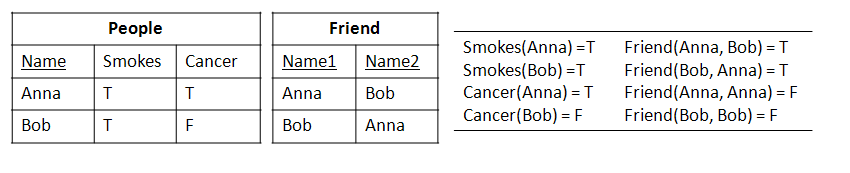
\includegraphics[width=1\textwidth]{database.png}
%}
\caption{A Bayesian/dependency template network (top) and the instantiated inference graphs (bottom). By convention, predicates (Boolean functors) are capitalized. Edges from the BN template are solid blue, while edges added by the BN-to-DN transformation are dashed black. The edge set in the DN comprises both solid and dashed arrows. Note that although the template BN (top) is acyclic, its  instantiation (bottom) features a bi-directed edge between $\it{gender}(bob)$ and $\it{gender}(anna)$. \label{fig:dn}
}
\end{center}
\end{figure} 
\subsection{Relational Dependency Networks}\label{sec:rdns}

Relational dependency networks~\cite{Neville2007} extend dependency networks to model distributions over multiple populations.
%There are various notations for defining random variables in relational structures.
%We adopt a functor-based notation from  a logic  for graphical-relational models \cite{Russell2010,Poole2003}. 
We  present the relational case using the parametrized random variable notation~\cite{Kimmig2014}.
A functor is a symbol denoting a function or predicate. Each functor has a set of values (constants) called the \defterm{domain} of the functor. Functors with Boolean ranges are called \textbf{predicates} and their name is capitalized. We consider only functors with finite domains. A first-order variable ranges over a domain of individuals.  An expression $\functor(\term_{1},\ldots,\term_{k})$, where $\functor$ is a functor 
and each $\term_{i}$ is a first-order variable or a constant, is a \defterm{Parametrized Random Variable} (PRV).
A directed acyclic graph whose nodes are PRVs is
a \defterm{parametrized Bayesian network structure}, while a general (potentially cyclic) directed graph whose nodes are PRVs is a \defterm{relational dependency network structure} (RDN). A parametrized Bayesian network structure or relational dependency network structure augmented with the appropriate conditional probabilities is  respectively a \defterm{parametrized Bayesian network template} or \defterm{relational dependency network template}.  
 %should fix this: the BN parameters are first-order only.
 Note that the RDN templates that we define in this paper have the same Markov blanket as the parametrized Bayesian network templates from which they are derived but a different edge structure and probabilities. Algorithm~\ref{alg:dnfeatures}, defined in Section~\ref{sect:learning}, converts the probabilities of the parametrized Bayesian template to their counterparts in the relational dependency template. 

RDNs extend dependency networks from \iid{} to relational data via knowledge-based model construction \cite{Neville2007}:
The first-order variables in a template RDN graph are instantiated for a specific domain of individuals to produce an {\em  instantiated} or {\em ground} propositional DN graph, the \defterm{inference graph}. It is typically assumed that the domains of the first-order variables are finite so that the inference graph is finite. For example, each individual in a finite domain may be named by a constant, and the constants are then used to instantiate the first-order variables~\cite[Sec.2.2.5]{Kimmig2014}. Figure~\ref{fig:dn} gives a dependency network template and its  inference graph. Given an edge in the template RDN, instantiating both the parent and the child of the edge with the same grounding produces an edge in the inference graph. An example local probability distribution for the graph in Figure~\ref{fig:dn} (abbreviating functors) is
$$P(\it{g(anna)}|\it{g(bob)}, \it{CD(anna)}, \it{F(anna,bob)},\it{F(bob,anna)},\it{F(anna,anna)}).$$

\paragraph{Language Bias.}
The general definition of a parametrized random variable allows PRVs to contain constants as well as population variables. For instance, both $\it{Friend}(\A,\B)$ and $\it{Friend}(\it{anna},\B)$ are valid PRVs. Another language extension is to allow parametrized random variables to be formed with aggregate functions, as described by Kersting and De Raedt \cite{Kersting2007}; see also \cite{Ravkic2015}. For example, it is possible to use a functor that returns the number of friends of a generic person $\A$. The main contribution of this paper, our relational BN-to-DN conversion method, can be used whether the parametrized random variables contain aggregates, constants, or only first-order variables. 
%A common restriction to simplify model structure learning is to exclude constants (e.g. \cite{Friedman99prm,Domingos2009}). Since this restriction applies only to the previous structure learning methods that we apply in this paper, we discuss it further in the parametrized Bayesian network learning section~\ref{sec:bnlearning} below. Friedman {\em et al.} investigated learning directed graphical models with aggregate functions \cite{Friedman99prm}. 


%\noindent Both the structure and the parameter space \fixneeded{Does ``parameter space'' refer to the database parameters or the statistical parameters?} of RDN models offer special advantages for relational data \cite{Neville2007,Natarajan2012}: 


%
%\fixneeded{Is there anything about the next paragraph that limits it to RDNs or does it all apply to DNs? If it applies to DNs, let's move it to DN section above.}
%\item Relational prediction  requires aggregating information from different linked individuals \cite{Natarajan2008}. \fixneeded{Give example of aggregation.}
%%Two common approaches are combining rules \cite{Kersting2007} and aggregation functions \cite{Getoor2007c}. 
%In a dependency network parameter, the aggregation encompasses the entire Markov blanket of a target node, whereas for Bayesian network parameters, the aggregation encompasses only part of the blanket.
%\end{enumerate}
%
%One of the challenges for inference on relational data is that, unlike the non-relational \iid{} case, {\em a single template node may be instantiated into multiple predictors} \cite{Natarajan2008}. In the inference graph of Figure~\ref{fig:dn}, each gender of a friend of $\it{anna}$ adds one relevant predictor for the value of $\it{gender}(anna)$. The number of predictors is therefore not fixed by the model, but depends on the number of individuals related to the target individual. Relational prediction therefore requires aggregating information from different linked individuals. Two common approaches are (i) combining rules \cite{Kersting2007} and (ii) aggregation functions \cite{Getoor2007c}. In a dependency network, the aggregation encompasses the entire Markov blanket of a target node, whereas in a Bayesian network, the aggregation encompasses only its parents.
%\fixneeded{Check if we still need this after full editing.}

\section{Learning Relational Dependency Networks via Bayesian Networks: Overview}\label{sect:learning}

From now on, almost all of our discussion concerns parametrized Bayesian networks and relational dependency networks. To shorten the discussion, we shall omit explicit mention of ``parametrized'' or ``relational'' and simply refer to Bayesian networks and dependency networks. If a particular point applies only to propositional networks, we mention this explicitly.

Our algorithm for rapidly learning relational dependency networks (Figure~\ref{fig:bn-flow})
begins with any relational learning algorithm for Bayesian networks. Using the resulting Bayesian network as a template, we then apply a simple, fast transformation to obtain a relational dependency template. Finally we apply a closed-form computation to derive the dependency network inference graph parameters from the Bayesian structure and parameters. %for computing a Gibbs probability using the log-linear equation.
\paragraph{BN-to-DN structure conversion.}
Converting a Bayesian network structure to a dependency network structure is simple: for each node, add an edge pointing to the node from each member of its BN Markov blanket~\cite{Heckerman2000}.  The result contains  bidirectional links between each node, its children, and its co-parents (nodes that share a child with this one). 
%
%This simply means adding edges into the node from each of its children and bidirectional links between the node and its co-parents (nodes that share a child with this one). 
This is equivalent to the standard moralization  method for converting a BN to an undirected model \cite{Domingos2009}, except that the dependency network contains bi-directed edges instead of undirected edges. Bi-directed edges permit  assigning different parameters to each direction, whereas undirected edges have only one parameter. 
\begin{figure}[t]
\begin{center}
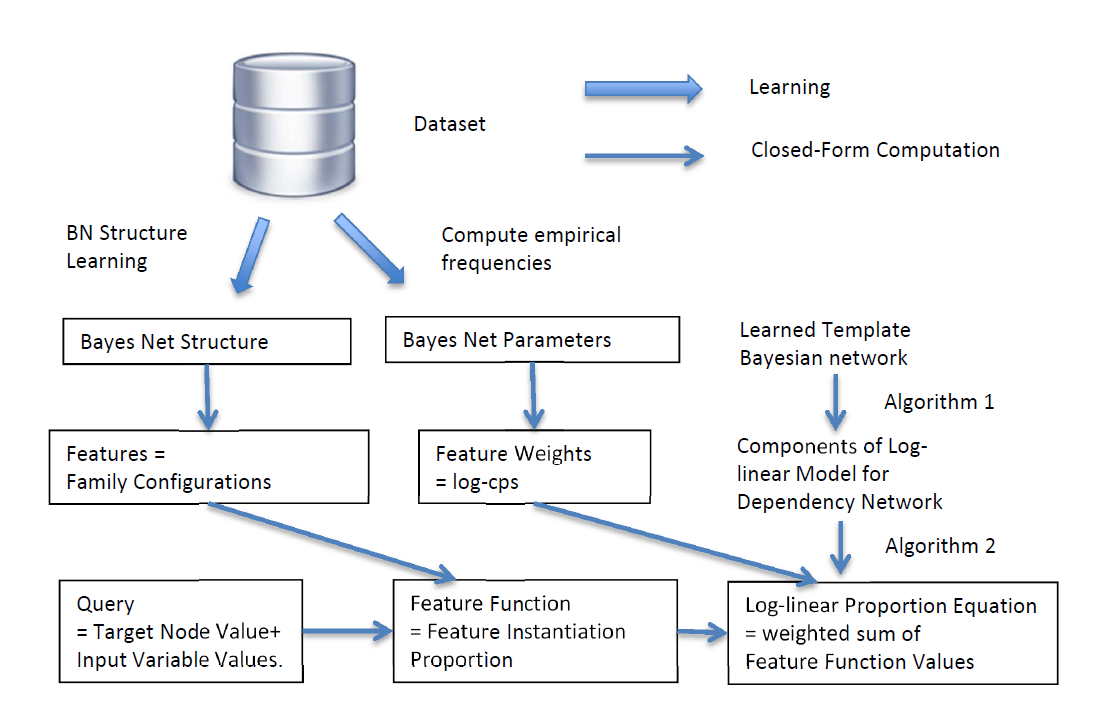
\includegraphics[width=0.7\textwidth]{bn-regress.png}
\caption{The program flow for computing local probability distributions from a template Bayesian network. Features and weights are computed from the Bayesian network. Feature function values are computed for each query. \label{fig:bn-flow}}
\end{center}
\end{figure}
\paragraph{BN-to-DN parameter conversion.}  For propositional data, converting Bayesian network parameters to dependency network parameters is simple: using the standard BN product formula for the joint distribution, solve for the local conditional probability distributions given Bayesian network parameters~\cite[Ch.14.5.2]{Russell2010}. A \defterm{family} comprises a node and its parents. A \defterm{family configuration} specifies a value for a child node and each of its parents. For example, in the template of Figure~\ref{fig:dn}~(top), one family is $\it{gender}(\A), \it{Friend}(\A,\B), \it{gender}(\B)$ and one of its eight possible configurations is
$$\it{gender}(\A) = \Man, \it{Friend}(\A,\B) = \true, \it{gender}(\B) = \Man.$$
The Markov blanket of a target node comprises multiple families, one each for the target node and each of its children, so
an assignment of values to the target's Markov blanket defines a unique configuration for each family. Hence in the propositional case the Markov blanket induces a {\em unique} log-conditional probability for each family configuration. The probability of a target node value given an assignment of values to the Markov blanket is then proportional to {\em the exponentiated sum of these log-conditional probabilities} \cite[Ch.14.5.2]{Russell2010}.

With relational data, however, different family configurations can be simultaneously instantiated, {\em multiple times.}  For example, the configuration $$\it{gender}(\A) = \Man, \it{Friend}(\A,\B) = \true, \it{gender}(\B) = \Man$$ has one instance for each pair of male friends $(a,b)$ (see also the example in Table~\ref{table:log-diff-example}).
We combine these multiple instantiations in a {\em log-linear model}, which defines a conditional random field for each target node. The general form of a discriminative log-linear model \cite{Sutton2007} is that the conditional probability of a target variable value given input variable values is proportional to an exponentiated weighted sum of feature functions. A feature function maps a complete assignment of ground node values (= target value + input variables) to a real number. 
We generalize the standard log-linear equation for i.i.d. data to define a relational log-linear equation following the pseudo code of Algorithm~\ref{alg:dnfeatures}. 


The features of the model are the family configurations (lines 3--6 of Algorithm~\ref{alg:dnfeatures}) where the child node is either the target node or one of its children. The feature weights are the log-conditional BN probabilities defined for the family configuration (lines 7--9) of Algorithm~\ref{alg:dnfeatures}). The feature functions are the family proportions, which is the number of times a relevant family configuration is instantiated, normalized by the total number of instantiations for that family. Without this standardization, features with more instantiations carry exponentially more weight. Ravkic {\em et al.} also use proportions for learning relational dependency networks~\cite{Ravkic2015}.

The next sections explain the details of the pipeline shown in Figure~\ref{fig:bn-flow}.
We begin at the beginning of the pipeline and review Bayesian network structure learning. Then we present the new contribution of this paper, the log-linear equation derived from the learned Bayesian network.

%by replacing the unique log-conditional probability with the {\em expected} log-conditional probability that results from selecting an instantiation of the family configuration uniformly at random. The probability of a target node value given an assignment of values to the Markov blanket is then proportional to the exponentiated sum of the expected log-conditional probabilites. %Without this normalization, features with more instantiations carry exponentially more weight. 
%The resulting closed-form equation defines a log-linear local probability distribution for the target node. Algorithm~\ref{alg:dnfeatures} provides pseudo-code for the transformation. 

\begin{algorithm}[htbp]
%\linesnumbered
\SetKwData{Calls}{Calls}
\SetKwData{Notation}{Notation}
\KwIn{Template Bayesian Network $\BN$ (Structure and Parameters)}
\KwOut{A List of Relevant Features; a Weight for each Feature }
\begin{algorithmic}[1]
\FOR{ each target node $\TT$}
\STATE{initialize $\it{Feature\_Weight}\_\it{List}(\TT)$ as the empty list}
	\FOR{ each $\UT$ in $\{ \Setaddterm{\TT} {\Ch{\TT}}\}$}
	\FOR {each value $\UV$ of the child node $\UT$ }
		\FOR {each vector of parent values $ \Prange{\UT}$}
			\STATE $\it{Feature}$ $F$  $:=$ $(\Appendterm{\UT  = \UV} {\Pa{\UT} = \Prange{\UT}})$ 
			\STATE  $\it{FeatureWeight} $ $\weight:=$ $\ln\cprob{\UT = \UV}{\Pa{\UT} = \Prange{\UT}}$
			\IF{the Feature $F$ does not contain a false relationship other than $\TT$}%, i.e. not relevant in $\BN$}
				\STATE{ add $(F , \weight)$ to $\it{Feature\_Weight}\_\it{List}(\TT)$  }
			\ENDIF \\	
		\ENDFOR
	\ENDFOR
\ENDFOR 
\ENDFOR
\STATE \Return {$\it{Feature\_Weight}\_\it{List}(\TT)$}
	%\STATE \Return $\Relfreq{C}{\DB}:=$ $\Relcount{C}{\DB}/\it{Total\_Relevant\_Count}$.
\end{algorithmic}
\caption{Computing Features and Weights for Template Dependency Network. \label{alg:dnfeatures}
}
\end{algorithm}



\section{Bayesian Network Learning for Relational Data} \label{sec:bnlearning}
We provide background on the previous work on learning Bayesian networks for relational data that we utilize in this paper. Readers may skip to ahead to the section on the log-linear equation for local probability distributions, presented in Section~\ref{sec:theequation}, without loss of continuity.
%
%
We review some of the fundamental insights and results from previous work concerning the scalability of Bayesian network learning, for both propositional and relational data. 
%Readers who are mainly interested in our empirical findings can skip this section without loss of continuity.


\subsection{Structure Learning} For structure learning, we used the learn-and-join (LAJ) algorithm \cite{Khosravi2010}. This is a state-of-the-art parametrized Bayesian network structure learning algorithm for relational data. It employs an iterative deepening search strategy similar to that introduced by Friedman {\em et al.} \cite{Friedman99prm}. 
We briefly review the main ideas behind the learn-and-join algorithm; for more details and examples please see \cite{Schulte2012}. 
The learn-and-join algorithm upgrades a single-table propositional BN learner for relational learning. The key idea of the algorithm can be explained in terms of the {\em table join lattice.} Recall that the (natural) join of two or more tables, written $\dtable_{1} \Join \dtable_{2} \cdots \Join \dtable_{k}$ is a new table that contains the rows in the Cartesian products of the tables whose values match on common fields. A table join corresponds to logical conjunction \cite{Ullman1982}.
%The join is a commutative and associative operation, so the join $\jtable_{1},\ldots,\jtable_{k}$ of a set of data tables is well-defined.
Say that a join table $\jtable$ is a \textbf{subjoin} of another join table $\jtable'$
%, %written $\jtable \sqsubseteq \jtable'$,
if $\jtable' = \jtable \Join \jtable^{*}$ for some join table $\jtable^{*}$. If $\jtable$ is a subjoin of $\jtable'$, then the fields (columns) of $\jtable$ are a subset of those in $\jtable'$. The subjoin relation defines the table join lattice. The basic idea of the learn-and-join algorithm is that join tables should inherit edges between descriptive attributes from their subjoins. This gives rise to the following constraints for two attributes $\node_{1}$, $\node_{2}$ that are both contained in some subjoin of $\jtable$. (i) $\node_{1}$ and $\node_{2}$ are adjacent in a BN $B_{\jtable}$ for $\jtable$ if and only if they are adjacent in a BN for some subjoin of $\jtable$. (ii) if all subjoin BNs of $\jtable$ orient the link as $\node_{1}\rightarrow\node_{2}$ resp. $\node_{1}\leftarrow\node_{2}$, then $B_{\jtable}$ orients the link as $\node_{1}\rightarrow\node_{2}$ resp. $\node_{1}\leftarrow\node_{2}$.
%\jtable \sqsubseteq\jtable'$, and $B_{\jtable}$ resp. $\B_{\jtable'}$ is a PBN for the attributes in $\jtable$ resp. $\jtable'$, and $\node_{1}, \node_{2}$ correspond to attributes in $\jtable$, then there is an edge $\node_{1} \rightarrow \node_{2}$ in $B_{\jtable}$ if and only if $\node_{1} \rightarrow \node_{2}$ is an edge in $\B_{\jtable'}$.
% need to handle the case where the subjoins don't all agree. Could I use Clark's NIPS algorithm to produce a consistent model. Here's the general picture: for each level, go through the points in the level, build a model for the point using the general model for s-1. Then merge the models at level s.
The learn-and-join algorithm then builds a PBN for the entire database $\D$ by level-wise search through the table join lattice. The user chooses a single-table BN learner. The learner is applied to table joins of size 1, that is, regular data tables. Then the learner is applied to table joins of size $s,s+1,\ldots$, where the constraints (i) and (ii) are propagated from smaller joins to larger joins.

\subsection{Computational Cost and Scalability} The computational cost of Bayesian network learning has been analyzed in previous work for both propositional and relational data. We review some of the main points as they pertain to the scalability of our overall BN-to-DN conversion approach.
The complexity analysis of the learn-and-join algorithm \cite{Schulte2012} shows that the key computational cost is the run-time of the propositional BN learner that is used as a subroutine in the algorithm. This cost in turn depends on two key factors: (1) Model search cost, the number of candidate models generated. (2) Model evaluation cost, the cost of evaluating a candidate model. The model evaluation cost is dominated by data access \cite{Moore1998}, especially the cost of computing sufficient statistics. In relational data, the sufficient statistics are the number of groundings that satisfy a formula in the input data~\cite{Friedman99prm,Domingos2009,Schulte2011}. This number is well-defined if we assume that each observed individual receives a unique name or ID in the data, such as a constant \cite{Kimmig2014}.
%, and that each first-order variable ranges over only finitely many observed individuals.  
We assume throughout the paper that the number of satisfying groundings is well-defined. We discuss each factor (1) and (2) in turn. 

\subsubsection{Model Search.}
While finding a Bayesian network that optimizes a model selection score is NP-hard~\cite{Chickering2004}, highly efficient local search methods have been developed that provide good approximations fast. The implementation of the LAJ algorithm that we used employs GES (Greedy Equivalence Search) as its propositional BN learning method. This search strategy has the remarkable property that in the sample size limit, it is guaranteed to find an optimal Bayesian network \cite{Chickering2002}. Thus as the sample size increases, the quality of the BN models discovered by GES increases as well, despite the NP-hardness of finding an optimal model. Given the language restriction of using only first-order variables and excluding constants, the number of models generated by relational BN model search is comparable to that generated by propositional BN model search \cite{Schulte2012}. Efficient relational BN model search with both constants and variables is to our knowledge an open problem. 

\subsubsection{Model Evaluation.} \label{sec:counting} Using the maximum likelihood scoring method, or other related scores, the fit of a Bayesian network to the input relational dataset can be evaluated in closed form given the sufficient statistics of the network \cite{Friedman99prm,Schulte2011}.  
%We discuss the complexity of this problem in Section~\ref{sec:complexity} below. 
While relational counting is not an easy problem, researchers have developed efficient solutions. These solutions find the number of instantiations of a relational feature much faster than by looping over all ground instances. Counting techniques for relational data include sorting tables on the attributes mentioned in the query \cite{Ullman1982,Graefe1998}, and {\em virtual join} algorithms that compute counts for conjunctive queries without enumerating all tuples that satisfy the query. Examples of virtual joins are tuple ID propagation, which stores intermediate counts along a relational pathway \cite{Yin2004}, and the fast M\"obius transform for queries that involve negated relationships \cite{Qian2014a}. A very recent approach reduces counting instantiations to computing the partition function for a suitable Markov network~\cite{Venugopal2015}.
 The important point for our experiments is that model evaluation by counting, which is most of what Bayes nets require, is much faster than iteratively computing model predictions for each ground fact in the input database, which is the standard model evaluation approach for other graphical model classes~\cite[Sec.8.5.1]{Neville2007}. 


\section{The Log-linear Proportion Equation} 
\label{sec:theequation}
We propose a log-linear equation, the \defterm{log-linear proportion equation} (lower right box of Figure~\ref{fig:bn-flow}), for computing a local probability distribution for a ground target node, $\FG{\TT}$, given 

\begin{enumerate}
\item a target value $\TV$ for the target node
\item a complete set of values $\QC$  for all ground terms other than the target node
\item a template Bayesian network
\end{enumerate}

The template structure is represented by functions that return the set of parent nodes of $\UT$, $\Pa{\UT}$, and the set of child nodes of $\UT$, $\Ch{\UT}$. The parameters of the template are
represented by the conditional probabilities of a node $\UT$ having a value $\UV$ conditional on the values of its parents, $$\cprob{\UT = \UV}{\Pa{\UT} = \Prange{\UT}}.$$ A grounding $\grounding$ substitutes a constant for each member of a list of first-order variables, $\{\A_{1} = \a_{1},\ldots, \A_{k} = \a_{k}\}$. Applying a grounding to a template node defines a fully ground target node: $\it{gender}(\A) \{\A = sam\} = \it{gender}(sam)$.  These are combined in the following log-linear equation to produce a local probability distribution:

%
\begin{definition}[The Log-Linear Proportion Equation]\label{def:log-diff-freq-eq}
\begin{eqnarray}
  \Gprob{\FG{{\TT}} = \TV} {\QC} &\propto &  \exp\\
  \notag
 \sum_{\UT} \sum_{\UV,\Prange{\UT}}   \quad \left[ \ln \cprob{\UT = \UV}{\Pa{\UT} = \Prange{\UT}} \right] &
    \cdot &
    \Relfreq{\Appendterm{\grounding;\UT  = \UV} {\Pa{\UT} = \Prange{\UT}}} {\Qconj}
%    \Relfreq{\Appendterm{\Ground{\UI}  = \UV} {\Ground{\Pa{\UI}} = \Prange{\UT}}} {\Qconj}
\end{eqnarray}
where 
\begin{eqnarray*}
%\UT &\mbox{varies over} &  \TT \mbox{and its children}; \\
\UT &\mathrm{varies\ over} & \Setaddterm{\{\TT\}} {\Ch{\TT}}; \\
\mbox{the singleton value} \ \UV & \mathrm{varies\ over} & \mbox{the range of}\  \UT;\\
\mbox{the vector of values} \ \Prange{\UT} & \mathrm{varies\ over} & \mbox{the product of the ranges of} \ \UT's\ \mbox{parents}, \\
& & \mbox{constrained to value} \ \TV \ \mbox{for occurrences of} \ \TT;\\
\grounding &\mathrm{grounds}& \mbox{template node }\TT;\\
\FG{\TT} &\mathrm{is} & \mbox{is the target ground node (i.e., } \FG{\TT} = \TT \grounding); \\
\mbox{and}~\Relevant{\Fvar} &\mathrm{is} & \mbox{the feature function, the family proportion}.
\end{eqnarray*}
\end{definition}
\newpage
The family proportion $\Relevant{\Fvar}$ is computed as follows:
%In terms of log-linear models, this corresponds to using family configurations as features and the {\em proportion of instantiations} that satisfy a family configuration as the feature function. 
\begin{enumerate}
\item For a given family configuration $(\Appendterm{\UT  = \UV} {\Pa{\UT} = \Prange{\UT}})$, let the \defterm{family  count} $$\Count{\Appendterm{\grounding;\UT  = \UV} {\Pa{\UT} = \Prange{\UT}}} {\Qconj}$$ be the number of instantiations that (a) satisfy the family configuration and the ground node values specified by $\Qconj$, and (b) are consistent with the equality constraint defined by the grounding $\grounding$.
%This notation is consistent with the parfactor notation of \cite{Poole2003}. 
\item The \defterm{relevant family count} $n^{r}$ is 0 if the family configuration contains a false relationship (other than the target node), else equals the family count. It is common in statistical-relational models to restrict predictors to existing relationships only \cite{Getoor2007c,Russell2010}.
\item The \defterm{family proportion} is the relevant family count, divided by the total sum of all relevant family counts for the given family:
{\scriptsize
\begin{equation} \notag
 \Relfreq{\Appendterm{\grounding;\UT  = \UV} {\Pa{\UT} = \Prange{\UT}}} {\Qconj} = \frac
 {\Relcount{\Appendterm{\grounding;\UT  = \UV} {\Pa{\UT} = \Prange{\UT}}} {\Qconj}}
 {\sum_{\UV',\Prange{\UT}'}\Relcount{\Appendterm{\grounding;\UT  = \UV'} {\Pa{\UT} = \Prange{\UT}'}} {\Qconj}
 }
\end{equation}
}
\end{enumerate}

In our experiments, family counts and proportions are computed using exact counting methods (see Section~\ref{sec:complexity} below). 

%specifies the proportion of instantiations that satisfy a given family configuration, relative to all family configurations with positive links only. 
%\paragraph{Example.}
%Table~\ref{table:log-diff-example} illustrates the computation of our log-linear model for predicting the gender of a new test instance ($sam$).

%\subsection{Example and Pseudocode}

\subsubsection{Example and Pseudo code.}


Table~\ref{table:log-diff-example} illustrates the computation of these quantities for predicting the gender of a new test instance ($sam$). 
%Algorithm~\ref{alg:dnfeatures} shows pseudocode for the closed-form transformation of Bayesian network structure and parameters into features and weights for the dependency network. 
Algorithm~\ref{alg:log-linear} shows pseudo code for computing the scores defined by the log-linear Equation~\eqref{def:log-diff-freq-eq}, given a list of weighted features and a target query. 


\begin{table}[tbhp]
\caption{Applying the log-linear proportion equation with the Bayesian network of Figure~\ref{fig:dn} to compute $\Gprob{\it{gender}(sam) = \Woman} {\QC}$ and $\Gprob{\it{gender}(sam) = \Man} {\QC}$. Each row represents a feature/family configuration. For the sake of the example we suppose that the conjunction $\QC$ specifies that Sam is a coffee drinker, has 60 male friends, and 40 female friends. $CP$ is the conditional probability BN parameter of Figure~\ref{fig:dn} and $\weight \equiv \ln(CP)$.
\label{table:log-diff-example}}
\centering
%\resizebox{1.1\textwidth}{!}{
\begin{tabular}{l@{\hspace{.2in}}l@{\hspace{.1in}}r@{\hspace{.1in}}r@{\hspace{.1in}}r@{\hspace{.1in}}r}
% This is a hand-computed example. 
{\setlength{\tabcolsep}{0pt}\begin{tabular}{l}Child \\Value $\UV$ \end{tabular}}&Parent State $\Prange{\UT}$&CP 
%$\cprob{\UT = \UV}{\Pa{\UT} = \Prange{\UT}}$
&{\setlength{\tabcolsep}{0pt}\begin{tabular}{c} $w$ \end{tabular}}&$\Relevant{\Fvar}$&{\setlength{\tabcolsep}{0pt}\begin{tabular}{c} $w \times \Relevant{\Fvar}$ \end{tabular}} \\\hline
$g(sam) = \Woman$&{\setlength{\tabcolsep}{0pt}\begin{tabular}{l}$ g(B) = \Woman,$\\ $F(sam,B) = \true$\end{tabular}}&$0.55$&$-0.60$&$0.4$&$-0.24$ \\
$g(sam) = \Woman$&{\setlength{\tabcolsep}{0pt}\begin{tabular}{l}$ g(B) = \Man,$\\ $ F(sam,B) = \true$\end{tabular}}&$0.37$&$-0.99$&$0.6$&$-0.60$ \\
$CD(sam) = \true$&{\setlength{\tabcolsep}{0pt}\begin{tabular}{l}$ g(sam) = \Woman$\end{tabular}}&$0.80$&$-0.22$&$1.0$&$-0.22$ \\
$CD(sam) = \false$&{\setlength{\tabcolsep}{0pt}\begin{tabular}{l}$g(sam) = \Woman$ \end{tabular}}&$0.20$&$-1.61$&$0.0$&$0.00$ \\\hline
\multicolumn{5}{l}{Sum ($\exp(Sum) \propto\Gprob{gender(sam)=\mathrm{\Woman}}{\QC}$)}&$-1.06$ \\\hline
$g(sam) = \Man$&{\setlength{\tabcolsep}{0pt}\begin{tabular}{l}$ g(B) = \Woman,$\\ $F(sam,B) = \true$\end{tabular}}&$0.45$&$-0.80$&$0.4$&$-0.32$ \\
$g(sam) = \Man$&{\setlength{\tabcolsep}{0pt}\begin{tabular}{l}$ g(B) = \Man,$\\ $ F(sam,B) = \true$\end{tabular}}&$0.63$&$-0.46$&$0.6$&$-0.28$ \\
$CD(sam) = \true$&{\setlength{\tabcolsep}{0pt}\begin{tabular}{l}$ g(sam) = \Man$\end{tabular}}&$0.60$&$-0.51$&$1.0$&$-0.51$ \\
$CD(sam) = \false$&{\setlength{\tabcolsep}{0pt}\begin{tabular}{l}$ g(sam) = \Man$\end{tabular}}&$0.40$&$-0.92$&$0.0$&$0.00$ \\\hline
\multicolumn{5}{l}{Sum ($\exp(Sum) \propto\Gprob{gender(sam)=\mathrm{\Man}}{\QC}$)}&$-1.11$ \\\hline

\end{tabular}
%}
\end{table}

%It is common in statistical-relational models to restrict predictors to existing relationships only \cite{Getoor2007c,Russell2010}.




\begin{algorithm}[htbp]
\SetKwData{Calls}{Calls}
\SetKwData{Notation}{Notation}
\KwIn{Feature-Weight List of Dependency Network, Query $ \Gprob{\FG{{\TT}} = \TV} {\QC}=?$. $\TT$ is a template node, $\FG{\TT} = \TT \grounding$ is the target grounding. }
%Feature $F = \Appendterm{\Ground{\UI}  = \UV} {\Ground{\Pa{\UI}} = \Prange{\UT}}$}
\KwOut{Normalized log-linear score}
\begin{algorithmic}[1]
%\FOR{ each target node $\TT$}
\STATE{initialize $\it{score}(\FG\TT = \TV) :=$ 0}
\FOR {each Feature $F = (\Appendterm{\UT  = \UV} {\Pa{\UT} = \Prange{\UT}})$ in  $\it{Feature\_Weight}\_\it{List}(
\TT)$}
\STATE  Let $\weight $ be the weight listed for feature $F$ 
\STATE \COMMENT{Next compute feature function.}
	\STATE   $\it{RelFamCnt}(F)$ $ :=$ $\Relcount{{\grounding}; \Appendterm{{\UI}  = \UV} {{\Pa{\UI}} = \Prange{\UT}}} {\Qconj}$
	\STATE $\it{TotalRelFamCnt}(U)$ := $\sum_{\UV',\Prange{\UT}'}\Relcount{ {\grounding}; \Appendterm{{\UI}  = \UV'} {{\Pa{\UI}} = \Prange{\UT}'}} {\Qconj}$
	\STATE  $\it{Family Proportion }$ $ \Relevant{\Fvar}(F) :=$ $\it{RelFamCnt}(F)/\it{TotalRelFamCnt}(U)$ \\
	\STATE   $\it{score}(\FG\TT = \TV)$ $\mathrel{+}= \Relevant{\Fvar}  \cdot  \weight $
\ENDFOR
\STATE \Return {Normalized scores for target node.}
\end{algorithmic}
%\label{alg:cpt}
\caption{Computing local probability distributions, the parameters of the Inference  Dependency Network. %\textbf{make notation consistent with ILP, not JAIR.} %Feature =  Family Configuration. 
\label{alg:log-linear}}
\end{algorithm}



\section{Discussion and Motivation} 

We discuss the key properties of our local distribution model, Equation~\eqref{def:log-diff-freq-eq}. We also provide a complexity analysis of the DN-to-BN conversion.

\subsection{Main Properties} We discuss the main properties that motivate our local distribution model. These are the following: (1) Log-linearity, (2) feature functions share a common standardized range, (3) nonrelational i.i.d. data are a special case, and (4) a random selection interpretation consistent with the probability logic of Halpern and Bacchus~\cite{Halpern90,Bacchus90,Schulte2014}.

\subsubsection{Log-Linearity.}
The survey by Kimmig {\em et al.} \cite{Kimmig2014} shows that most statistical-relational methods define log-linear models.  Khazemi {\em et al.} have shown that many relational aggregators can be represented by a log-linear model with suitable features \cite{Kazemi2014}. 
Equation~\eqref{def:log-diff-freq-eq} instantiates this well-established log-linear schema as follows.

\begin{description}
\item[The model features] are the family configurations $(\Appendterm{\UT  = \UV} {\Pa{\UT} = \Prange{\UT}})$ where the child node is either the target node or one of its children.
\item[The feature weights]  are the log-conditional BN probabilities defined for the family configuration. 
\item[The input variables] are the values specified for the ground (non-target) nodes by the conjunction $\QC$.
\item[The feature functions] are the family proportion $\Relevant{\Fvar}$. 
\end{description}

%that specify the values of a child node and its parents in the template Bayesian network, 
%The feature weights are the log-conditional BN probabilities defined for the family configuration. The input variables are the values specified for the ground (non-target) nodes by the conjunction $\QC$.
%The family count specifies how many times the feature is instantiated in the input variables (plus the target node value).
%The feature functions are the family proportion $\Relevant{\Fvar}$.
%
 Like other log-linear relational models, Equation~\ref{def:log-diff-freq-eq} enforces parameter tying, where different groundings of the same family configuration receive the same weight~\cite{Kimmig2014}. In the related work section~\ref{sec:related} we compare Equation~\ref{def:log-diff-freq-eq} to other log-linear models such as Markov Logic networks.

\subsubsection{Standardization.} Using proportions as feature functions has the desirable consequence that the range of all feature functions is standardized to [0,1]~\cite{Ravkic2015}. It is well-known that the number of instantiation counts in relational data can differ for different families, depending on the population variables they contain. This ill-conditioning causes difficulties for log-linear models because families with more population variables can have an exponentially higher impact on the score prediction \cite{Lowd2007}. Intuitively, counts tacitly conflate number of instantiations with degree of information. Proportions avoid such ill-conditioning.


\subsubsection{Generalizing the Propositional Case.} An important general design principle is that {\em relational learning should have  i.i.d. learning as a special case}~\cite{Ch.10deraedt,Knobbe2006}: When we apply a relational model to a single \iid{} data table, it should give the same result as the propositional model. Equation~\ref{def:log-diff-freq-eq} satisfies this principle. In the propositional case, an assignment of values to all nodes other than the target node specifies a {\em unique} value for each family configuration. This means that all the family counts $n^{r}$ are either 0 or 1, hence all relevant proportions $p^{r}$ are 0 or 1, depending on whether a family configuration matches the query or not. For a simple illustration, consider the edge $\it{gender}(\A) \rightarrow \it{CoffeeDr}(\A)$. Since this edge concerns only the $\it{Person}$ domain associated with the single population variable $\A$, we may 
view this edge as a propositional sub-network.
%
%the structure $\it{gender} \rightarrow \it{CoffeeDr}$ as a propositional subnetwork. 
Suppose the query is $P(\it{gender}(sam)= \Woman|\it{CoffeeDr}(sam)=\true)$. The only family configurations with nonzero counts are $\it{gender}(sam)= \Woman$ (count 1) and $\it{CoffeeDr}(sam)=\true),\it{gender}(sam)= \Woman$ (count 1). Equation~\eqref{def:log-diff-freq-eq} gives


\begin{eqnarray*}
P(\it{g}(sam)= \Woman|\it{CD}(sam)=\true) \propto \\
\exp \{\ln P(\it{g}(sam)= \Woman) + \ln P(\it{CD}(sam)=\true)|\it{g}(sam)= \Woman)\}.&&
\end{eqnarray*}

%$\Relcount$

This agrees with the i.i.d. BN formula for a local conditional probability, which is the product of the BN conditional probabilities for the target node given its children, and the target node's children given their parents (cf. Section~\ref{sect:learning}). 
%This formula can be derived from the BN product rule for defining a joint probability \cite[Ch.14.5.2]{Russell2010}. 
In our simple two-node example, the formula can be derived immediately from Bayes' theorem:

\begin{eqnarray*}
P(\it{g}(sam)= \Woman|\it{CD}(sam)=\true) \propto \\
P(\it{CD}(sam)=\true)|\it{g}(sam)= \Woman) \times P(\it{g}(sam)= \Woman),&&
\end{eqnarray*}

\noindent which agrees with the solution above derived from Equation~\eqref{def:log-diff-freq-eq}. It may seem surprising that in predicting gender given coffee drinking, the model should use the conditional probability of coffee drinking given gender. However, Bayes' theorem entails that $P(X|Y)$ is always proportional to $P(Y|X)$. In our example, given that the BN model specifies that women are more likely to be coffee drinkers than men, the information that Sam is a coffee drinker raises the probability that Sam is a woman. 

\subsubsection{Random Selection Interpretation.}

The inner sum of Equation~\eqref{def:log-diff-freq-eq} computes the expected log-conditional probability for a family with child node $\UT$, when we randomly select a relevant grounding of the first-order variables in the family. The equation is therefore consistent with the random selection semantics established in classic AI research by Halpern and Bacchus \cite{Halpern90,Bacchus90,Schulte2014}. 
%cite workshop paper as well
The expected log-conditional probability may be defined as follows. Fix a BN family with child node $\UT$ and parents $\Pa{\UT}$. 
Let $\grounding'$ be a grounding of the nodes in the family, that is consistent with the target grounding $\grounding$. 
The conjunction $\Qconj$ specifies a unique value $\UT \grounding' = \UV^{\Qconj} $ for each ground child node $\UT \grounding'$. It also specifies a unique value $\Pa{\UT} \grounding'= \Prange{\UT}^{\Qconj}$ for each ground parent set $\Pa{\UT} \grounding'$. Let $G$ be the set of all relevant groundings consistent with the target grounding, that is, the family configuration defined by the grounding is relevant. 

Using this notation, the \defterm{expected log-conditional probability} from a randomly selected relevant grounding for the family is given by

\begin{equation}\label{eq:random-select}
\frac{1}{|G|} \sum_{\grounding' \in G} \ln \cprob{\UT \grounding' = \UV^{\Qconj}}{\Pa{\UT} \grounding' = \Prange{\UT}^{\Qconj}}.
\end{equation}

The next proposition asserts that the equivalence of random selection with the log-linear proportion equation:

\begin{proposition} \label{prop:random}
The expected log-conditional probability is the same as the contribution of each family in the log-linear sum of the equation in Definition~\ref{def:log-diff-freq-eq}:

\begin{align*}
\frac{1}{|G|} \sum_{\grounding' \in G} \ln \cprob{\UT \grounding' = \UV^{\Qconj}}{\Pa{\UT} \grounding' = \Prange{\UT}^{\Qconj}} 
= 
\\
 \sum_{\UT} \sum_{\UV,\Prange{\UT}}   \quad \left[ \ln \cprob{\UT = \UV}{\Pa{\UT} = \Prange{\UT}} \right] 
 \cdot 
\Relfreq{\Appendterm{\grounding;\UT  = \UV} {\Pa{\UT} = \Prange{\UT}}} {\Qconj}.
\end{align*}

\end{proposition} 

A formal proof is in Section~\ref{sec:random-proof}. Fundamentally the proposition holds because the expected value of a sum of terms is the sum of expectations of the terms.





\subsection{Complexity of Algorithms 1 and 2} \label{sec:complexity}
%\paragraph{Computing Features and Feature Weights} 
The loops of Algorithm~\ref{alg:dnfeatures} enumerate every family configuration in the template Bayesian network exactly once. Therefore {\em computing features and weights takes time linear in the number of parameters of the Bayesian network.} 

Evaluating the log-linear equation, as shown in Algorithm~\ref{alg:log-linear}, requires finding the number of instantiations that satisfy a conjunctive family formula, given a grounding. This is an instance of the general problem of computing the number of instantiations of a formula in a relational structure. Computing this number is a well-studied problem  with highly efficient solutions, which we discussed in Section~\ref{sec:counting}. To analyze the computational complexity of counting,  a key parameter is the number $m$ of first-order variables that appear in the formula~\cite{Vardi1995}. A loose upper bound on the complexity of counting instantiations is $d^{m}$, where $d$ is the maximum size of the domain of the first-order variables. Thus counting instantiations has parametrized polynomial complexity \cite{Flum2006}, meaning that if $m$ is held constant, counting instantiations requires polynomially many operations in the size of the relational structure (i.e., the size of $\Qconj$ in Equation~\eqref{def:log-diff-freq-eq}). For varying $m$, the problem of computing the number of formula instantiations is \#P-complete \cite[Prop.12.4]{Domingos2007}.


 
 
%The Bayesian network  parameters can be estimated using the empirical conditional frequencies observed in an input dataset $\FG{\Delta}$: The parameter estimate for a family configuration is the number of instantiations of that family configuration in $\FG{\Delta}$, divided by the sum of all instantiation counts for that family that agree on the parent values and vary the child values. In our notation, the estimate is defined by
%
%\newcommand{\CTPa}{\Count{\Appendterm{\TT = \TV} {\Pa{\TT} = \Prange{\TT}}}  {\FG{\Delta}}}
%\newcommand{\CTPb}{\Count{\Appendterm{\TT = \TV'} {\Pa{\TT} = \Prange{\TT}}}  {\FG{\Delta}}}
%
%\begin{equation} \label{eq:frequencies}
%\estcprob{\TT = \TV} {\Pa{\TT} = \Prange{\TT}} {\FG{\Delta}} = 
%    \frac{\CTPa}
%           {\sum_{\TV' \in \Range{\TT}}\CTPb}.
%\end{equation}
%
%A theoretical justification for using the observed conditional frequencies is that these estimates maximize a pseudo-likelihood function that measures how well a template BN matches an input dataset \cite{Schulte2011,Schulte2013}. The pseudo-likelihood can be interpreted as the expected value of the log-likelihood of a random grounding of the BN nodes in the template model.
%
%Although this theoretical justification assures us of the conceptual coherence of Equation~\ref{def:log-diff-freq-eq}, the ultimate test is whether the method can achieve comparable accuracy and greater speed than prior methods of computing relational dependency networks. In the next section, we empirically compare these methods.

\section{Consistency of the Derived Dependency Networks} \label{sec:consistency} A basic question in the theory of dependency networks is the {\em consistency} of the local probabilities.  Consistent local probabilities ensure the existence of a single joint probability distribution $p$ that induces the various local conditional probability distributions $P$ for each node
$$\Gprob{\FG{\TT} = \TV} {\QC} \propto p(\FG{\TT} =\TV,\QC)$$  
for all target nodes $\FG{\TT}$ and query conjunctions $\QC$~\cite{Heckerman2000}.

We present a precise condition on a template Bayesian network for its resulting dependency network to be consistent and the implications of those conditions.  An  template Bayesian network is \defterm{edge-consistent} if every edge has the same set of population variables on both nodes.

\begin{theorem}\label{th:consistent-dn}
A template Bayesian network is edge-consistent if and only if its derived dependency network is consistent.
\end{theorem}

%
%The primary inconsistency result is the following theorem:
%
%\begin{theorem}\label{theorem:inconsistency-condition}
%Assume that a template BN contains at least one edge $e_1$ such that the parent and child do not contain the same set of population variables. Then there exists an edge $e_2$ (which may be the same as or distinct from $e_1$) from parent $\TT_{1}$ to child $\TT_{2}$, ground nodes $\FG{\TT_{1}}$ and $\FG{\TT_{2}}$,  and a query conjunction $\QC$ such that: the ground nodes $\FG{\TT_{1}}$ and $\FG{\TT_{2}}$ have mutually inconsistent conditional distributions $\cprob{\FG{\TT_{1}}}{\QC}$ and $\cprob{\FG{\TT_{2}}}{\QC}$ as defined by Equation~\ref{def:log-diff-freq-eq}.
%\end{theorem}

The proof of this result is complex, so we present it in an appendix (Section~\ref{sec:consistency-proof}). Intuitively, in a joint distribution, the correlation or potential of an edge 
is a single fixed quantity, whereas in Equation~\eqref{def:log-diff-freq-eq}, the correlation is adjusted by the size of the relational neighbourhood  of the target node, which may be either the child or the parent of the edge. If the relational neighborhood size of the parent node is different from that of the child node, the adjustment makes the conditional distribution of the child node inconsistent with that of the parent node. The edge-consistency characterization shows that the inconsistency phenomenon is properly relational, meaning it arises when the network structure contains edges that relate parents and children from different populations.

%This theorem has several implications. First, it implies necessary and sufficient conditions on a template Bayes net for its derived dependency network to be consistent. We define an \defterm{edge-consistent template Bayesian network} to be a network for which every edge has the same set of population variables on both nodes.
%
%\begin{corollary}\label{corollary:consistent-dn}
%A template Bayesian network is edge-consistent if and only if its derived dependency network is consistent.
%A relational dependency network constructed from a Bayesian network is consistent if and only if the relevant family counts are the same for each ground node in the 
%\end{corollary}
%\begin{proof}

%As Figure~\ref{fig:dn} shows, the ground RDN structure defines a ground Markov network when bidirected edges are replaced by undirected edges (cf. \cite{Heckerman2000}). Ground families are cliques in the ground Markov network. In that case, let $N$ be the common relevant family count. To a family configuration $(\Appendterm{\FG{\UT}  = \UV} {\FG{\Pa{\UT}} = \Prange{\UT}})$, we may assign the clique potential 
%$\cprob{\UT = \UV}{\Pa{\UT} = \Prange{\UT}}^{1/N}.$ The conditional distributions for this Markov network are then exactly those defined by the log-linear equation~\ref{def:log-diff-freq-eq}. 

%On the other hand, without an equality constraint on relevant family counts, an RDN derived from a BN is generally not consistent. A sufficient and necessary condition for when different relevant counts may occur with different ground nodes is that a parent and a child contain different population variables.
%
%\end{proof}

The edge-consistency condition required by this theorem is quite restrictive: Very few template Bayesian networks will have exactly the same set of population variables on both sides of each edge.\footnote{A commonly used weaker condition is range-restriction: that the population variables in the child node should be contained in the population variables of its parents \cite{Kersting2007}, but not vice versa as with edge-consistency.}
%also add reference to Jesse's hybrid dependency paper
%The propositional case is an important exception:
%
%\begin{corollary}\label{corollary:propositional-consistency}
%A propositional template Bayesian network will always have a consistent derived dependency network.
%\end{corollary}
%\begin{proof}
%A propositional template Bayesian network has exactly one population variable, therefore it is always edge-consistent.
%\end{proof}
%
Therefore relational template Bayesian networks, which have multiple population variables, will most often produce inconsistent dependency networks. None of the Bayesian networks learned for our benchmark datasets (see Section~\ref{sec:empirical-comparison}) is edge-consistent, and therefore, by Theorem~\ref{th:consistent-dn},  the resulting dependency networks are inconsistent.

\paragraph{Inference with Inconsistent Dependency Networks.}
 Previous work has shown that dependency networks learned from data are almost always inconsistent but nonetheless provide accurate predictions using Gibbs sampling. The general idea is to apply the local probability distributions in the dependency network to update the values of each variable in turn~\cite{Heckerman2000,Neville2007,Lowd2012}. One approach is ordered pseudo-Gibbs sampling: fix an ordering of the random variables and update each in the fixed order. Heckerman \etal{} show that  
 ordered pseudo-Gibbs sampling defines a Markov chain with a unique stationary joint distribution over the random variables \cite[Th.3]{Heckerman2000}. A recent approach was developed for Generative Stochastic Networks, where the next variable to be updated is chosen randomly, rather than according to a fixed ordering. Bengio shows that this procedure too defines a Markov chain with a unique stationary joint distribution over the random variables \cite[Sec.3.4]{Bengio2014}. Lowd discusses further methods for inference with inconsistent dependency networks~\cite{Lowd2012}.

% The consistency constraints on the dependency networks derived using our methods have an interesting implication for the class of models representable by such networks:

% \begin{corollary}\label{corollary:distinct-models}
% The relational dependency network produced by grounding a template dependency network derived from a template Bayes net are a different model class than the dependency networks
% \end{corollary}
% \begin{proof}
% Mumble consistency of networks comparable to Markov networks but our networks are inconsistent mumble ...
% \end{proof}

%\begin{figure}[htbp]
%\begin{center}
%%\resizebox{0.78\textwidth}{!}{
%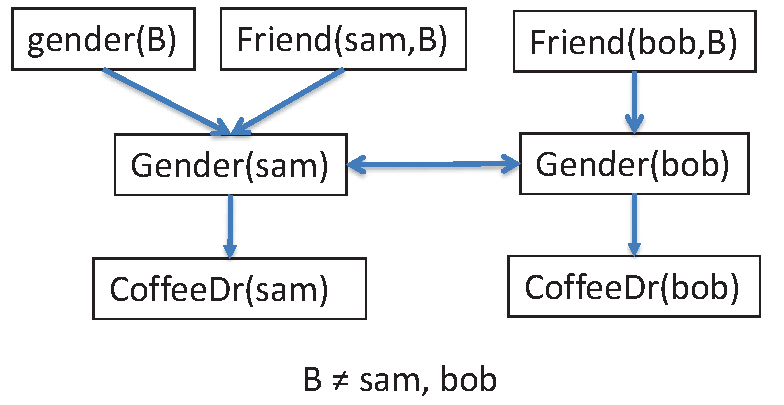
\includegraphics[width = 0.7 \textwidth]{figures/pdn}
%%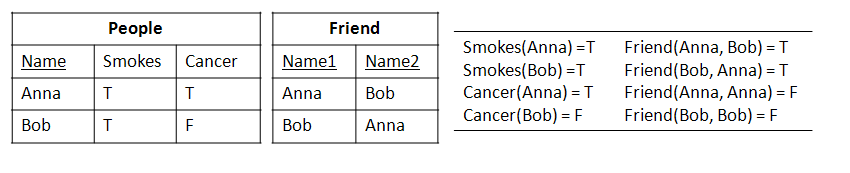
\includegraphics[width=1\textwidth]{database.png}
%%}
%\caption{Partially ground graph. \label{fig:partial-nn}}
%\end{center}
%\end{figure}
%
%Figure~\ref{fig:partial-nn} shows a partially ground graph with assignments $\it{gender}(bob) = \Man$ and $\it{gender}(sam) = \Man$. 
%% \marginpar{Zhensong: please insert figure as we discussed}.
% Assume that both Bob and Sam have the same number of friends, say 50, and are friends with each other. Then in predicting the gender of Bob, the bidirected edge between them contributes to Equation~\ref{def:log-diff-freq-eq} the term $\cprob{\it{gender}(\A) = \Man}{\it{gender}(\B)=\Man}^{1/50} = 0.63^{1/50}$. Similarly, in predicting the gender of Sam, the bidirected edge contributes the term $0.63^{1/50}$. This is consistent with assigning a clique potential of $0.63^{1/50}$ when the clique that contains both $\it{gender}(bob)$ and $\it{gender}(sam)$ specifies both to be men. In contrast, suppose that Bob has 50 friends and Sam has 100. Then in predicting the gender of Bob, the bidirected edge contributes the term $0.63^{1/50}$, but in predicting the gender of Sam, the bidirected edge now contributes the term $0.63^{1/100}$. There is no single joint clique potential that contributes different terms to a log-linear equation depending on which node is chosen as the target node. Intuitively, in a joint distribution, the strength of the correlation between Sam being a man and Bob being a man is a single fixed quantity, whereas in Equation~\ref{def:log-diff-freq-eq}, the correlation is adjusted by the size of the relational neighbourhood of Sam reap. Bob.

\section{Empirical Evaluation: Design and Datasets}\label{sec:empirical-comparison}
There is no obvious baseline method for our RDN learning method because ours is the first work that uses the approach of learning an RDN via a Bayesian network. Instead we benchmark against the performance of our method a different approach for learning RDNs, which uses an ensemble learning approach based on functional gradient boosting. Boosted functional gradient methods have been shown to outperform previous methods for learning relational dependency networks \cite{Khot2011,Natarajan2012}. 
%
%Our argument is not that the Bayes net approach is superior to boosting on all or even most datasets. The two approaches are very different, with  different strengths and limitations. Our view is that  ultimately the best system for learning RDNs is one that combines the strengths of Bayesian network learning with those of boosting. After we present our experimental results in detail, we make suggestions for how this combination can be achieved. Despite the fundamental differences in approach, we believe that our empirical comparison provides enough evidence that Bayesian network learning (together with the variables-only language bias) brings substantial scalability advantages, while at the same the predictive accuracy of the learned dependency networks is competitive with that of the boosting networks. Therefore the advantages in scalability and interpretability establish Bayesian network conversion as a worthwhile option for learning relational dependency networks.  
%
%We compare learning RDNs via Bayesian networks with learning via boosted functional gradient methods. Boosting methods follow the traditional approach to learning dependency networks, which is to learn a collection of separate discriminative models, one for each node in the network \cite{Heckerman2000}. 
%Boosted functional gradient methods have been shown to perform well on small datasets \cite{Khot2011,Natarajan2012}; our experiments extend these results to medium--large datasets. 
%\subsection{Experimental Conditions and Metrics}\label{sec:conditions}

All experiments were done on a machine with 8~GB of RAM and a single Intel Core~2 QUAD Processor Q6700 with a clock speed of 2.66~GHz (there is no hyper-threading on this chip), running Linux Centos 2.6.32. Code was written in Java, JRE 1.7.0. All code and datasets are available~\cite{bib:jbnsite}. 
\subsubsection{Datasets}
We used six benchmark real-world databases. For more details please see the references in \cite{Schulte2012}. Summary statistics are given in Table~\ref{table:learning-times}.   The large datasets with over 1M tuples are orders of magnitude larger than what has been analyzed by previous methods. The number of parametrized random variables, usually between 9-19, is at the upper end of what has been analyzed previously in statistical-relational learning. In the future work section we discuss scaling Bayesian network learning to even more complex relational datasets.


\begin{description}

\item[UW-CSE] This dataset \cite{Kok2005a} lists facts about the Department of Computer Science and Engineering at the University of Washington.\footnote{http://alchemy.cs.washington.edu/data/uw-cse/}  There are two entity classes (278 Persons, 132 Courses) and two relationships (AdvisedBy, TaughtBy). There are six descriptive attributes, of average arity 3.8. The experiments reported in \cite{Natarajan2012} used the same dataset; their version is available in WILL format.\footnote{http://pages.cs.wisc.edu/~tushar/Boostr/datasets/uw.zip}

\item[MovieLens] MovieLens is a  commonly-used rating dataset.\footnote {www.grouplens.org} We added more related attribute information about the actors, directors and movies from the Internet Movie Database (IMDb) (www.imdb.com, July 2013).
It contains two entity sets, Users and Movies. The User table has 3 descriptive attributes, $\age$, $\it{gender}$, and $\it{occupation}$. We discretized the attribute $\age$ into three equal-frequency bins. There is one relationship table Rated corresponding to a Boolean predicate. The Rated table contains Rating as descriptive attribute. For each user and movie that appears in the database, all available ratings are included. MovieLens(1M) contains 1~M ratings, 3,883 Movies, and 6,039 Users. MovieLens(0.1M) contains about 0.1~M ratings, 1,682~Movies, and 941~Users. We did not use the binary genre predicates because they are easily learned with exclusion rules. 


\item[Mutagenesis] This dataset is widely used in inductive logic programming research. 
It contains information on 4893 Atoms, 188 Molecules, and Bonds between them. We use the discretization of Schulte and Khosravi~\cite{Schulte2012}. Mutagenesis has two entity tables, $\it{Atom}$ with 3 descriptive attributes of average arity 4, and $\it{Mole}$, with %188 entries and
5 descriptive attributes of average arity 5, including two attributes that are discretized into ten values each (logp and lumo). It features two relationships $\it{MoleAtom}$ indicating which atoms are parts of which molecules, and $\it{Bond}$ which relates two atoms and has 1 descriptive attribute of arity 5. 

\item[Hepatitis] This data is a modified version of the PKDD02 Discovery Challenge database. %, which includes removing tests with null values. 
The database contains information on the laboratory examinations of hepatitis B and C infected patients. It contains data on the laboratory examinations
of hepatitis B and C infected patients. The examinations were realized between 1982 and 2001 on 771 patients. The data are organized in 7 tables (4 entity tables,  3 relationship tables and 16 descriptive attributes). They contain basic information about the patients, results of biopsy, information on interferon therapy, results of out-hospital examinations, results of in-hospital examinations. The average arity of all descriptive attributes is 4.425.

\item[Mondial] Data from multiple geographical Web data sources. There are two entity classes, 185 Countries and 135 Types of Economies. There are 5 descriptive attributes for each entity class, with average arity 4.4 for Country and 4.6 for Economy Type. A Borders relationship indicates which country borders which. The Economy relationship relates a country to a type of economy.

\item[IMDb] %copy from sigmod paper.
The largest dataset in terms of number of total tuples (more than 1.3M) and schema complexity. %attributes.
It combines MovieLens %\footnote{www.grouplens.org, 1M version} 
with data from the Internet Movie Database (IMDb)\footnote{www.imdb.com, July 2013} \cite{Peralta2007}. There are 98,690 Actors, with 2 descriptive attributes of average arity 4;  2,201 Directors, with 2 descriptive attributes of average arity 5.5; 3,832 Movies, with 4 descriptive attributes of average arity 3.5; and 996,159 ratings. 
\end{description}

\subsubsection{Methods Compared} \label{sec:methods} Functional gradient boosting is a state-of-the-art method for applying discriminative learning to build a generative graphical model. The local discriminative models are  ensembles of relational regression trees \cite{Khot2011}. Functional gradient boosting for relational data is implemented in the Boostr system~\cite{Khot2013}.
 For functors with more than two possible values, we followed \cite{Khot2011} and converted each such functor to a set of binary predicates by introducing a predicate for each possible value.
%The current implementation does not support multi-class boosting, so following previous experiments \cite{Khot2011}, we limited our comparison to {\em binary predicates}, i.e., functors that can take on only two possible values (e.g., $\it{AdvisedBy}$). \textbf{probably need to change this, see Cathy}
%
We compared the following methods:
\begin{description}
\item[RDN\_Bayes] Our method: Learn a Bayesian network, then convert it to a relational dependency network. 
\item[RDN\_Boost] The RDN learning mode of the Boostr system \cite{Natarajan2012}. 
%Information from ground nodes linked to the target is aggregated with functions $count, max, average$ and existential quantification .
\item[MLN\_Boost] The MLN learning mode of the Boostr system. It takes a  list of target predicates for analysis. We provide each binary predicate in turn as a single target predicate, which amounts to using MLN learning to construct an RDN. This RDN uses a log-linear model for local probability distributions that is derived from Markov Logic Networks.
\end{description}
%Used as an RDN learner in this way, the main difference of MLN\_Boost with RDN\_Boost is that it aggregates information from ground nodes that are linked to the target node using a log-linear model derived from Markov Logic Networks. 
The measurements reported below used the default Boostr settings, with one exception: We decreased the number of regression trees in the ensemble from the default 20 to 10. This led to a small reduction in learning time, but did not decrease the predictive accuracy because on our datasets, Boostr does not produce more than 10 different trees. For other settings, similar changes from Boostr's default changed neither accuracy nor learning time noticeably.

For Bayesian network structure learning, we used the implementation by the creators of the LAJ algorithm, which is available on-line \cite{bib:jbnsite}. It is important to note that this implementation incorporates a language bias (cf. Section~\ref{sec:methods}): it considers only parametrized random variables without any constants, that is, first-order variables only. This is a common restriction for statistical-relational structure learning methods (e.g. \cite{Friedman99prm,Domingos2009,Ravkic2015}),  which trades off expressive power for faster learning. For Bayesian network parameter estimation, we used maximum likelihood estimates, computed with previous methods~\cite{Qian2014a}.


%\paragraph{Estimating Bayesian network parameters.}
%The Bayesian network parameters can be estimated by applying the maximum likelihood principle, which entails using the empirical conditional frequencies observed in an input relational database \cite{Schulte2011,Schulte2014}. 
% Although there is theoretical justification for using the empirical frequencies, the ultimate test is whether the method can achieve comparable accuracy and greater speed than prior methods of computing relational dependency networks. In the next section, we empirically compare these methods.

%A similar use of Bayesian network learning is made by Schulte and Khosravi \cite{Schulte2012} where the Bayesian network learned by the LAJ algorithm is converted to a Markov Logic Network for performing inference. That paper converted only the model structures. The difference to this paper is that we convert the Bayesian network to a dependency network, not to a Markov network, and that we convert the BN to DN parameters as well. Our Theorem 1 entails that the relational dependency networks we obtain from BN-to-DN conversion are not in general equivalent to Markov Logic Networks.

%To obtain the BN structure for RDN\_Bayes, the learn-and-join algorithm~\cite{Schulte2012} was applied to each benchmark database. %The resulting structure and parameters were used for all methods in this experiment. 

\subsubsection{Prediction Metrics}
We follow \cite{Khot2011} and evaluate the algorithms using conditional log likelihood (CLL) and area under the precision-recall curve (AUC-PR). AUC-PR is appropriate when the target predicate features a skewed distribution as is typically the case with relationship predicates. %These metrics have been used in previous evaluations of MLN learning~\cite{Domingos2007,Schulte2012}.  
For each fact $\FG{\TT} = \TV$ in the test dataset, we evaluate the accuracy of the predicted local probability $\Gprob{\FG{\TT} = \TV} {\QC}$, where $\QC$ is a complete conjunction for all ground terms other than $\FG{\TT}$. Thus $\QC$ represents the values of the input variables as specified by the test dataset.
%For classification accuracy, a model's prediction is scored as correct if the true value of the ground term in the test dataset receives the highest Gibbs probability. 
CLL is the average of the logarithm of the local probability for each ground truth fact in the test dataset, averaged over all test predicates. For the gradient boosting method, we used the AUC-PR and likelihood scoring routines included in Boostr.
%Thus $\exp(CLL)$ is the geometric mean of the Gibbs probabilities.\footnote{The geometric mean of a list of numbers $x_{1},\ldots,x_{n}$ is $(\prod_{i} x_{i})^{1/n}$.} 


Both metrics are reported as means and standard deviations over {\em all binary predicates}.\footnote{Most of the results reported in the boosting paper \cite{Khot2011} give accuracy metrics for one or two predicates only.}
The learning methods were evaluated using 5-fold cross-validation. Each database was split into 5 folds by randomly selecting entities from each entity table, and restricting the relationship tuples in each fold to those involving only the selected entities  (i.e., subgraph sampling~\cite{Schulte2012}). The models were trained on 4 of the 5 folds, then tested on the remaining one. 
%All results are over the 5~folds, over all descriptive attributes in the database. 

\section{Results} 
% results are from multiple-link/ILP2014/ilp14_Nov26.xlsx
%


We report learning times and accuracy metrics. In addition to these quantitative assessments, we inspect the learned models to compare the relational features represented in the model structures. Finally we make suggestions for combining the strengths of boosting with the strengths of Bayesian network learning. 


\subsection{Learning Times.} Table~\ref{table:learning-times} shows learning times for the methods. The Bayesian network  learning simultaneously learns a joint model for all parametrized random variables (PRVs). The PRVs follow the language bias of the LAJ algorithm and contain functors and population variables only (cf. Section~\ref{sec:methods}). 
%[Recall that Boolean PRVs are predicates.] 
For the boosting method, we added together the learning times for each target PRV. 
%The total learning times are not directly comparable because Bayesian network  learning simultaneously learns a joint model for all predicates. We therefore report total learning time divided by the number of all predicates for RDN\_Bayes, and total learning time divided by the number of binary predicates for the boosting methods.
On MovieLens(1M), the boosting methods take over 2~days to learn a classifier for the relationship $\it{B\_U2Base}$, so we do not include learning time for this predicate for any boosting method.
On the largest database, IMDb, the boosting methods cannot learn a local distribution model for the three relationship predicates with our system resources, so we only report learning time for descriptive attributes by the boosting methods. Likewise, our accuracy results in Tables~\ref{table:cll} and~\ref{table:AUC} include measurements for only descriptive attributes on the datasets IMDb and MovieLens(1M).
%\textbf{Cathy: need to add bold}

\begin{table}[tb]
  \addtolength{\tabcolsep}{2pt}
  \centering
  \caption{Learning Time. The total learning time for constructing a relational dependency network from an input database. Only partial boosting learning times are reported for the larger databases MovieLens(1M) and IMDb---see text for details. Spread is reported as coefficient of variation (CV---standard deviation / mean). PRV = Parametrized Random Variable.\label{table:learning-times}}
\begin{tabular}{l r r @{\hspace{20pt}} r r r r r r }\hline
             &           &             &  \multicolumn{2}{c}{RDN\_Bayes} & \multicolumn{2}{c}{RDN\_Boost} & \multicolumn{2}{c}{MLN\_Boost}\\
                                               \cline{4-5}                                  \cline{6-7}                                  \cline{8-9}
Dataset & \begin{tabular}{c}\#Tuples/\\1000 \end{tabular} & PRVs & (s) & CV & (s) & CV & (s) & CV \\\hline
UW & 0.6 & 14 & \textbf{14} & 0.00 & 237 & 0.06 & 329 & 0.16 \\
Mondial & 0.9 & 18 & 1836 & 0.07 & \textbf{369} & 0.06 & 717 & 0.05 \\
Hepatitis & 11.3& 19 & 5434 & 0.01 & 6648 & 0.02 & \textbf{3197} & 0.04 \\
Mutagenesis & 24.3& 11 & \textbf{11} & 0.00 & 1342 & 0.04 & 1040 & 0.02 \\
MovieLens(0.1M) & 83.4& 7 & \textbf{8} & 0.07 & 3019 & 0.04 & 3292 & 0.01 \\
MovieLens(1M) & 1010.1& 7/6 & \textbf{8} & 0.09 & 32230 & 0.04 & 25528 & 0.04 \\
IMDb & 1538.4& 17/13 & \textbf{9346} & 0.22 & 78129 & 0.04 & 29704 & 0.03 \\\hline
\end{tabular}
\end{table}
 % Table generated by Excel2LaTeX from sheet 'learning time table May 12'
%\begin{table}[htbp]
%  \centering
%  \caption{Learning Time (Sec) Per Predicate}
%    \begin{tabular}{|l|p{2cm}|r|r|r|r|}
%\hline
%     Dataset & all predicates / binary predicates & \# tuples & RDN\_Bayes & RDN\_Boost & MLN\_Boost \\ \hline
%    UW    & 14/4  & 612   & 0.74$\pm$0.05 & 14.57$\pm$0.39 & 19.27$\pm$0.77  \\
%    Mondial & 18/4  & 870   & 101.53$\pm$6.90 & 27.21$\pm$0.98 & 41.97$\pm$1.03 \\
%    Hepatitis & 19/7  & 11,316 & 285.71$\pm$20.94 & 250.61$\pm$5.32 & 229.73$\pm$2.04  \\
%    Mutagenesis & 11/6  & 24,326 & 0.70$\pm$0.02 & 117.70$\pm$6.37 & 48.65$\pm$1.34 \\ 
%    MovieLens(0.1M) & 7/2   & 83,402 & 1.11$\pm$0.08 & 2638.71$\pm$272.78 &  1866.605$\pm$112.54\\
%    MovieLens(1M) & 7/2   & 1,010,051 & 1.12$\pm$0.10 & $>$24 hours & $>$24 hours \\ \hline
%  
%    \end{tabular}%
%  \label{table:learning-times}%
%\end{table}%
%
%
%\begin{table}[htbp]
%  \centering
%  \caption{Learning Time (Sec) Per Predicate}
%    \begin{tabular}{|l|p{2cm}|r|r|r|r|}
%\hline
%     Dataset & all predicates / binary predicates & \# tuples & RDN\_Bayes & RDN\_Boost & MLN\_Boost \\ \hline
%    UW    & 14/4  & 612   & 0.74$\pm$0.05 & 14.57$\pm$0.39 & 19.27$\pm$0.77  \\
%    Mondial & 18/4  & 870   & 101.53$\pm$6.90 & 27.21$\pm$0.98 & 41.97$\pm$1.03 \\
%    Hepatitis & 19/7  & 11,316 & 285.71$\pm$20.94 & 250.61$\pm$5.32 & 229.73$\pm$2.04  \\
%    Mutagenesis & 11/6  & 24,326 & 0.70$\pm$0.02 & 117.70$\pm$6.37 & 48.65$\pm$1.34 \\ 
%    MovieLens(0.1M) & 7/2   & 83,402 & 1.11$\pm$0.08 & 2638.71$\pm$272.78 &  1866.605$\pm$112.54\\
%    MovieLens(1M) & 7/2   & 1,010,051 & 1.12$\pm$0.10 & $>$24 hours & $>$24 hours \\ \hline
%  
%    \end{tabular}%
%  \label{table:learning-times}%
%\end{table}%
Consistent with other previous experiments on Bayesian network learning with relational data~\cite{Khosravi2010,Schulte2012}, Table~\ref{table:learning-times} shows that RDN\_Bayes scales very well with the number of data tuples: even the MovieLens dataset with 1~M records can be analyzed in seconds. 
%This is because it provides closed-form parameter estimation and hence closed-form model scoring. 
RDN\_Bayes scales worse with the number of PRVs, since it learns a joint model over all PRVs simultaneously,  although the time  remains feasible (1--3 hours for 17--19 predicates; see also \cite{Schulte2012}). By contrast, the boosting methods scale well with the number of predicates, which is consistent with findings from  propositional learning \cite{Heckerman2000}.
%\cite{Heckerman2000,Hulten2003}.
Gradient boosting scales much worse with the number of data tuples.
 % because 
 %model evaluation itself is quite expensive for the boosting methods. 
% Unlike propositional (\iid{}) data, relational data are represented in multiple tables, so evaluation requires expensive combining of information from different tables \cite{Neville2007}. 
% Consequently, learning Bayesian networks explores a more complex model space than learning RDNs using the boosting approaches, but is typically much faster due to its more efficient model evaluation.
% Table originally generated by Excel2LaTeX from sheet 'CLL'
% Since modified to move standard deviations to end and improve formatting
{\addtolength{\tabcolsep}{2pt}
\begin{table}[tb]
  \centering
  \caption{Conditional Log-Likelihood: Mean (top), Std. Dev. (bottom) }
    \begin{tabular}{l r r r r r r r}
    \hline
                 &          &              &                 &          & \multicolumn{2}{c}{MovieLens} & \\
                                                                                 \cline{6-7}
    Method & UW    & Mond. & Hepa. & Muta. & (0.1M) & (1M) & IMDb \\
    \hline
    RDN\_Boost & -0.30 & -0.48 & -0.48 & -0.36  & -0.50 & \textbf{-0.22} & \textbf{-0.49} \\
    MLN\_Boost & -0.14 & -0.40 & -0.49 & -0.23 & -0.50 & -0.23 & \textbf{-0.49} \\
    RDN\_Bayes & \textbf{-0.01} & \textbf{-0.25} & \textbf{-0.39} & \textbf{-0.22} & \textbf{-0.30} & -0.28 & -0.51 \\
    \hline
    RDN\_Boost & 0.02 & 0.03 & 0.01 & 0.02 & 0.01 & 0.00 & 0.00 \\
    MLN\_Boost & 0.01 & 0.05 & 0.01 & 0.02 & 0.01 & 0.00 & 0.00 \\
    RDN\_Bayes & 0.00 & 0.06 & 0.10 & 0.07 & 0.00 & 0.00 & 0.00 \\
    \hline
    \end{tabular}%
  \label{table:cll}%
\end{table}%
}
% Table originally generated by Excel2LaTeX from sheet 'AUC-PR'
% Since modified to move standard deviations to end and improve formatting
\begin{table}[tb]
  \addtolength{\tabcolsep}{2pt}
  \centering 
  \caption{Area Under Precision-Recall Curve: Mean (top), Std. Dev. (bottom).}
    \begin{tabular}{c r r r r r r r}    \hline
                 &          &            &          &           & \multicolumn{2}{c}{MovieLens} & \\
                                                                          \cline{6-7}     
    Method & UW    & Mond. & Hepa. & Muta. & (0.1M) & (1M)                            & IMDb\\
    \hline
    RDN\_Boost &0.42&0.27&0.55&0.71&0.50&0.88&0.63 \\
    MLN\_Boost &0.68&0.44&0.55& \textbf{0.86} &0.50&0.88&0.63 \\
    RDN\_Bayes & \textbf{0.89} & \textbf{0.79} &0.55&0.50& \textbf{0.65} &\textbf{1.00}& \textbf{0.85} \\
    \hline
    RDN\_Boost &0.00&0.00&0.01&0.02&0.01&0.00&0.01 \\
    MLN\_Boost &0.01&0.04&0.01&0.04&0.01&0.00&0.01 \\
    RDN\_Bayes &0.00&0.07&0.11&0.10&0.02&0.00&0.00 \\
    \hline
    \end{tabular}%
  \label{table:AUC}%
\end{table}%
%
%\begin{table}[htbp]
% \centering
%  \caption{Average Conditional Log-Likelihood. \textbf{Zhensong: please make chart as in presentation.}}
%    \begin{tabular}{|r|r|r|r|r|r|r|r|} \hline
%    \textbf{CLL} & UW    & Mondial  & Hepatitis & Mutagenesis  & MovieLens(0.1M) \\ \hline
%   RDN\_Boost & -0.29$\pm$0.02 & -0.48$\pm$0.03 & -0.51$\pm$0.00 & -0.43$\pm$0.02 & -0.58$\pm$0.05 \\
%    MLN\_Boost & -0.16$\pm$0.01 & -0.40$\pm$0.05 & -0.52$\pm$0.00 & -0.24$\pm$0.02 & -0.38$\pm$0.06 \\
%    RDN\_Bayes & \textbf{-0.01$\pm$0.00} & \textbf{-0.25$\pm$0.06} & \textbf{-0.39$\pm$0.10} & \textbf{-0.22$\pm$0.07} & \textbf{-0.30$\pm$0.02} \\ \hline
%    \end{tabular}%
%  \label{table:cll}%
%%\end{table}%
%
%% Table generated by Excel2LaTeX from sheet 'temp'
%%\begin{table}[htbp]
% \centering 
% \caption{Average Area Under Precision-Recall Curve}
%    \begin{tabular}{|r|r|r|r|r|r|} \hline
%    \textbf{AUC-PR} & UW    & Mondial  & Hepatitis & Mutagenesis  & MovieLens(0.1M) \\ \hline
%    RDN\_Boost & 0.32$\pm$0.01 & 0.27$\pm$0.01 & \textbf{0.71$\pm$0.02} & 0.63$\pm$0.02 & 0.52$\pm$0.03 \\
%    MLN\_Boost & 0.52$\pm$0.01 & 0.44$\pm$0.05 & \textbf{0.71$\pm$0.02} & \textbf{0.83$\pm$0.05} & 0.52$\pm$0.05 \\
%    RDN\_Bayes & \textbf{0.89$\pm$0.00} & \textbf{0.79$\pm$0.07} & 0.55$\pm$0.11 & 0.50$\pm$0.10 & \textbf{0.65$\pm$0.02} \\ \hline
%    \end{tabular}%
%  \label{table:AUC}%
%\end{table}%

%
%\begin{table}[!htb]
%    %\caption{P-values for two-tailed pair-wise t-test}
%    \begin{minipage}{.5\linewidth}
%      \caption{ two-tailed  t-test  on CLL}
%      \centering
%        \begin{tabular}{|l|r|r|} \hline
%    \textbf{p-value} &RDN\_Boost   &MLN\_Boost    \\ \hline
%    MLN\_Boost &0.026  &             \\
%    RDN\_Bayes & 0.002 & 0.014  \\ \hline
%    \end{tabular}%
%  \label{table:ttestcll}%
%    \end{minipage}%
%    \begin{minipage}{.5\linewidth}
%      \centering
%        \caption{ two-tailed  t-test  on AUC-PR. \textbf{Zhensong: please fill in the t-test table}}
%       \begin{tabular}{|l|r|r|} \hline
%    \textbf{p-value} &RDN\_Boost   &MLN\_Boost    \\ \hline
%    MLN\_Boost &0.072  &             \\
%    RDN\_Bayes & 0.297 & 0.631  \\ \hline
%    \end{tabular}%
%  \label{table:ttestpr}%
%    \end{minipage} 
%\end{table} 
% 
%Tables~\ref{table:cll} and~\ref{table:AUC} show results for predictive accuracy. Table~\ref{table:ttest} shows that these results are statistically significant at $p < 0.05$. \textbf{Need to fill in details of test, fill in numbers.} 
%Our system resources did not suffice for evaluating the metrics on MovieLens(1M).  
\subsection{Accuracy} Whereas learning times were evaluated on all PRVs, unless otherwise noted, we evaluate accuracy on the binary PRVs  only (e.g., $\it{gender},\it{Borders}$), because the boosting methods are based on binary classification. By the likelihood metric (Table~\ref{table:cll}), the Bayesian network method performs best on four datasets, comparably to MLN\_Boost on Mutagenesis, and slightly worse than both boosting methods on the two largest datasets. By the precision-recall metric (Table~\ref{table:AUC}), the Bayesian network method performs substantially better on four datasets, identically on Hepatitis, and substantially worse on Mutagenesis.

Combining these results, for most of our datasets the Bayesian network method has comparable accuracy and much faster learning. This is satisfactory because boosting is a powerful method that achieves accurate predictions by producing a tailored local model for each target predicate. By contrast, Bayesian network learning simultaneously constructs a joint model for all predicates, and uses simple maximum likelihood estimation for parameter values. Also, Boostr searches a more expressive feature space that allows constants as well as first-order variables.
We conclude that \emph{Bayesian network  learning with first-order variables only, scales much better to large datasets, and provides competitive accuracy in predictions.} 
 
\subsection{Comparison of Model Structures} 
%The fundamental reason why Bayesian network learning is faster than classifier ensemble learning is that the cost of model evaluation remains: Bayesian networks can be scored against the data in closed-form, requiring only sufficient statistics. Dependency networks in contrast require a pass through each ground instance of a target node, and each relational neighborhood of the ground instance. The inventors of RDNs noted this as a fundamental scalability challenge for RDN learning \cite{Neville2007}. This is a reversal compared to i.i.d. data where learning dependency networks is faster than learning Bayesian networks \cite{Hulten2003,Heckerman2000}. This reversal occurs because accessing relational data stored in multiple tables is more expensive than accessing i.i.d. data stored in a single table. For larger relational datasets, the smaller data access cost of Bayesian network learning outweighs the higher model search cost from using a more complex generative rather than discriminative model.

%\paragraph{Scalability.} OS
% There are several possibilities for increasing the speed of the RDN-Boost system: (1) Change parameter settings to restrict the search space. For example, although we decreased the number of trees learned to 10, many of the learned trees are still redundant. (2) Implement an early stopping scheme for RDN-Boost, to adapt the number of trees, the maximum length of a clause, and other settings to a specific dataset. (3) Use auxilliary data structures such as Hoeffding trees \cite{Lopes2009}. A promising topic for future work is to leverage the speed of Bayesian network learning to improve functional gradient boosting; we discuss this under future work.
 
Boosting is known to lead to very accurate classification models in general \cite{Bishop2006}. For propositional data, a Bayesian network classifier with maximum likelihood estimation for parameter values is a reasonable baseline method \cite{Grossman2004}, but we would expect more accuracy from a boosted ensemble of regression trees. Therefore the predictive performance of our RDN models is not due to the log-linear equation~\eqref{def:log-diff-freq-eq}, but due to the more powerful features that Bayesian network learning finds in relational datasets. These features involve longer chains of relationships than we observe in the boosting models. Kok and Domingos emphasize the importance of learning clauses with long relationship chains \cite{Kok2010}. The ability to find complex patterns involving longer relationship chains comes from the lattice search strategy, which in turn depends on the scalability of model evaluation in order to explore a complex space of relationship chains. Table~\ref{table:mb-comparison} reports results that quantitatively confirm this analysis. 

For each database, we selected the target PRV where RDN-Bayes shows the greatest predictive advantage over RDN-Boost (shown as $\Delta$ CLL and $\Delta$ AUC-PR). We then compute how many more PRVs the RDN-Bayes model uses to predict the target predicate than the RDN-Boost model, shown as $\Delta$ Predicates. This number can be as high as 11 more PRVs (for Mondial). We also compare how many more population variables are contained in the Markov blanket of the RDN-Bayes model, shown as $\Delta$ Variables. In terms of database tables, the number of population variables measures how many related tables are used for prediction in addition to the target table. This number can be as high as 2 (for IMDb and Hepatitis). To illustrate Figure~\ref{fig:dn-structure} shows the parents (Markov blanket) of target node $\it{gender}(\U)$ from IMDb in the RDN-Boost and RDN-Bayes models. The RDN-Bayes model introduces 4 more parents and 2 more variables, $\it{Movie}$ and $\it{Actor}$. These two variables correspond to a relationship chain of length 2. Thus BN learning discovers that the gender of a user can be predicted by the gender of actors that appear in movies that the user has rated.
\begin{table}[!htb]
 \addtolength{\tabcolsep}{5pt}
 \caption{Difference in Markov blankets between RDN\_Bayes and RDN\_Boost. $\Delta x$ = ($x$ for RDN\_Bayes - $x$ for RDN\_Boost).  RDN\_Bayes predicts a target more successfully because it uses more  predicates and those predicates contain more first-order variables.}
      \centering
\begin{tabular}{l l c c c c}
\hline
Database & Target & $\Delta$ Predicates  & $\Delta$ Vars. & $\Delta$ CLL & $\Delta$ AUC-PR \\\hline
Mondial & religion & 11 & 1 & 0.58 & 0.30\\
%IMDb & gender & 6 & 2 & 0.3 & 0.68 \\
IMDb & gender & 4 & 2 & 0.30 & 0.68 \\
UW-CSE & student & 4 & 1 & 0.50 & 0.55 \\
Hepatitis & sex & 4 & 2 & 0.20 & 0.25\\
Mutagenesis & ind1 & 5 & 1 & 0.56 & 0.22 \\
MovieLens & gender & 1 & 1 & 0.26 & 0.26 \\\hline
\end{tabular}
 \label{table:mb-comparison}%
\end{table}% 

\begin{figure}[htbp]
\begin{center}
%\resizebox{0.78\textwidth}{!}{
%\includegraphics[width=1\textwidth]{figures/dn-structure}
\includegraphics[width=1\textwidth]{dn-structure}
%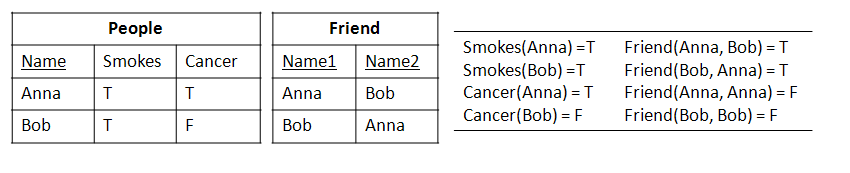
\includegraphics[width=1\textwidth]{database.png}
%}
\caption{The parents of target $\it{gender}(\U)$ in the models discovered by RDN\_Boost~(left) and RDN\_Bayes~(right). \label{fig:dn-structure}}
\end{center}
\end{figure}
%% Table generated by Excel2LaTeX from sheet 'temp'
%\begin{table}[htbp]
%  \centering
%  \caption{Add caption}
%    \begin{tabular}{|r|r|r|r|r|r|}
%    \hline
%    dababase & \# of functor in MB & \# extra first order variable & CLL-diff & PR-diff & target node  \\
%    \hline
%    imdb  & 8/2   & 3/0   & 0.30  & 0.68  & u\_gender\_f  \\
%    \hline
%    uw    & 4/0   & 1/0   & 0.50  & 0.55  & student\_0  \\
%    \hline
%    hep   & 6/2   & 2/0   & 0.20  & 0.25  & sex\_0  \\
%    \hline
%    mondial & 11/0  & 1/0   & 0.58  & 0.30  & class\_0  \\
%    \hline
%    muta  & 5/0   & 1/0   & 0.56  & 0.22  & ind1\_0  \\
%    \hline
%    movielens & 2/1   & 1/0   & 0.26  & 0.26  & Gender\_M  \\
%    \hline
%    \end{tabular}%
%  \label{tab:addlabel}%
%\end{table}%
%

%; as the inventors of the boosting method put it, ``we sacrifice comprehensibility for better predictive performance'' \cite{Natarajan2012}. 

\section{Combining Bayesian Network Learning and Gradient Boosting} \label{sec:combine}

Gradient Boosting is a very different approach from Bayesian network conversion, in several respects: (1) Different model type: single-model Bayesian network vs. ensemble of regression trees. (2) Different language bias: the learn-and-join structure learning algorithm considers nodes with population variables only, whereas a novel aspect of structure learning with the boosting methods is that they allow both variables and constants. (3) Different learning methods: local heuristic search to optimize a model selection score, vs. boosting. 

Given these fundamental differences, it is not surprising that our experiments show different strengths and limitations for each approach. Strengths of Bayes nets include: (1) Speed through fast model evaluation, which facilities exploring complex cross-table correlations that involve long chains of relationships. (2) Interpretability of the conditional probability parameters. (3) Learning easily extends to attributes with more than two possible values.
Strengths of boosting include: (1) Potentially greater predictive accuracy through the use of an ensemble of regression trees. (2) Exploring a larger space of statistical-relational patterns that include both first-order variables and constants. 
These two approaches can be combined in several natural ways to benefit from their mutual strengths.

\begin{description}
\item [Feature Selection] Fast Bayesian network learning methods can be used to select features. Regression tree learning should work much faster when restricted to the BN Markov blanket of a target node. The mode declaration facility of the Boostr system supports adding background knowledge about predictive predicates. For nodes whose BN Markov blankets contain disjoint features, boosting can be applied in parallel on disjoint datasets.\footnote{We owe this point to an anonymous reviewer for the Machine Learning journal.}
%This would facilitate exploring longer relationship chains within the boosting framework.
\item [Initialization] The Bayesian network can provide an initial dependency network for the boosting procedure. 
%
%Gradient boosting can be used in place of maximum likelihood estimation to improve the conditional probability models. 
Gradient boosting can be applied to improve the estimate of the Bayesian network parameters (node conditional distribution given parents) or of the dependency network parameters (node conditional distribution given parents). It is well-known that decision trees can improve the estimation of Bayesian network parameters~\cite{Friedman1998}; a tree ensemble should provide an even more accurate model. 
Using boosting for local probability models would leverage its ability to learn statistical patterns with constants rather than first-order variables only.
\item [Proportions not Counts] Functional gradient boosting can be used with proportions as feature functions rather than counts, to avoid ill-conditioned learning with feature functions of different magnitudes. 
%cite Davis on hybrid dependency networks 
\end{description}


%\begin{enumerate}
%\item Fast Bayesian network learning methods can be used to select features. Regression tree learning should work much faster when restricted to the BN Markov blanket of a target node. The mode declaration facility of the Boostr system supports adding background knowledge about predictive predicates. For nodes whose BN Markov blankets contain disjoint features, boosting can be applied in parallel on disjoint datasets.\footnote{We owe this point to an anonymous reviewer for the Machine Learning journal.}
%%This would facilitate exploring longer relationship chains within the boosting framework.
%\item The Bayesian network can provide an initial dependency network for the boosting procedure. 
%%
%%Gradient boosting can be used in place of maximum likelihood estimation to improve the conditional probability models. 
%Gradient boosting can be applied to improve the estimate of the Bayesian network parameters (node conditional distribution given parents) or of the dependency network parameters (node conditional distribution given parents). It is well-known that decision trees can improve the estimation of Bayesian network parameters~\cite{Friedman1998}; a tree ensemble should provide an even more accurate model. 
%Using boosting for local probability models would leverage its ability to learn statistical patterns with constants rather than first-order variables only.
%\item Functional gradient boosting can be used with proportions as feature functions rather than counts, to avoid ill-conditioned learning with feature functions of different magnitudes. 
%%cite Davis on hybrid dependency networks 
%\end{enumerate}


\section{Related Work} \label{sec:related}
Dependency networks were introduced by Heckerman et al.~\cite{Heckerman2000} and extended to relational data by Neville and Jensen~\cite{Neville2007}. 
Heckerman et al. compare Bayesian, Markov and dependency networks for nonrelational data~\cite{Heckerman2000}. Neville and Jensen compare Bayesian, Markov and dependency networks for relational data, including the scalability advantages of Bayesian network learning~\cite[Sec.8.5.1]{Neville2007}. Using the parametrized random variable formalisms, Kimmig \etal{} compare prominent statistical-relational formalisms, for example Relational Bayesian networks, Bayes Logic Programs, and Markov Logic Networks~\cite{Kimmig2014}.

\emph{Bayesian networks.} There are several proposals for defining directed relational template models, based on graphs with directed edges or rules in clausal format \cite{Kersting2007,Getoor2007c}. Defining the probability of a child node conditional on multiple instantiations of a parent set requires the addition of combining rules \cite{Kersting2007} or aggregation functions \cite{Getoor2007c}. 
%As described by \cite{Kersting2007}, aggregate functions can be added to a Parametrized Bayesian network by including functor nodes with aggregates. 
Combining rules such as the arithmetic mean~\cite{Natarajan2008} combine global parameters with a local scaling factor, as does our log-linear Equation~\eqref{def:log-diff-freq-eq}. In terms of combining rules,  our equation uses the {\em geometric mean} rather than the arithmetic mean.\footnote{The geometric mean of a list of numbers $x_{1},\ldots,x_{n}$ is $(\prod_{i} x_{i})^{1/n}$. %The logarithm of the geometric mean is therefore $1/n \sum_{i} \ln x_{i}$. 
Thus geometric mean = exp(average (logs)).} To our knowledge, the geometric mean has not been used before as a combining rule for relational data.  
Another difference with template Bayesian networks is that the geometric mean is applied to the entire Markov blanket of the target node, whereas usually a combining rule applies only to the parents of the target node. 

\emph{Markov Networks.} Markov Logic Networks (MLNs) provide a logical template language for undirected graphical models. 
Richardson and Domingos propose transforming a Bayesian network to a Markov Logic network using moralization, with log-conditional probabilities as weights \cite{Domingos2009}. 
This is also the standard BN-to-MLN transformation recommended by the Alchemy system \cite{bib:bayes-convert}. A discriminative model can be derived from any MLN \cite{Domingos2009}.  The structure transformation was used in previous work \cite{Schulte2012}, where MLN parameters were learned, not computed in closed-form from BN parameters. The local probability distributions derived from an MLN obtained from converting a Bayesian network are the same as those defined by our log-linear Formula~\ref{def:log-diff-freq-eq}, {\em if} counts replace proportions as feature functions \cite{Schulte2011}. Since the local probability distributions derived from an MLN are consistent, our main Theorem~\ref{th:consistent-dn} entails that in general, there is no MLN whose log-linear local models are equivalent to our log-linear local models with  proportions as feature functions.  Schulte \etal{} report empirical evidence that using proportions instead of counts, with the Bayesian network features and parameters, substantially improves predictive accuracy substantially~\cite{Schulte2012d}.
 

\section{Conclusion and Future Work} 
\label{sec:conclusion}
Relational dependency networks offer important advantages for modelling relational data. They can be learned quickly by first learning a Bayesian network, then performing a closed-form transformation of the Bayesian network to a dependency network. The key question is how to transform BN parameters to DN parameters. We introduced a relational generalization of the standard propositional BN log-linear equation for the probability of a target node conditional on an assignment of values to its Markov blanket. The new log-linear equation uses a sum of expected values of BN log-conditional probabilities, with respect to a random instantiation of first-order variables. This is equivalent to using feature instantiation proportions as feature functions.  Our main theorem provided a necessary and sufficient condition for when the local log-linear equations for different nodes are mutually consistent. On six benchmark datasets, learning RDNs via BNs scaled much better to large datasets than state-of-the-art functional gradient boosting methods, and provided competitive accuracy in predictions.

{\em Future Work.}
The boosting approach to constructing a dependency network by learning a collection of discriminative models is very different from learning a Bayesian network. There are various options for hybrid approaches that combine the strengths of both. (1) Fast Bayesian network learning can be used to select features. Discriminative learning methods should work faster restricted to the BN Markov blanket of a target node. (2) The Bayesian network can provide an initial dependency network structure. Gradient boosting can then be used to fine-tune local distribution models. 

One of the advanced features of the boosting system is including relational features that involve individual constants, not only first-order variables. Extending structure learning for parametrized Bayesian networks to include nodes with constants is an open problem. 
% could cite ourselves late breaking AAAI
This would also permit an apples-to-apples comparison of the speed of Bayesian network learning vs. boosting using a compatible language bias.

Several important applications, such as large-scale information extraction from web pages \cite{Zhang2015}, require analyzing datasets with many more parametrized random variables than the benchmarks in our experiments. One approach to modelling massive numbers of random variables is to upgrade the propositional Bayesian network learning algorithms that are designed for such datasets, for instance the Sparse Candidate algorithm \cite{friedman99:_learn_bayes}. 


\section*{Acknowledgements} 
We are indebted to the reviewers and participants of StarAI~2012 and ILP~2014 for helpful comments on earlier drafts and presentations. Anonymous reviewers for the Machine Learning journal provided extensive suggestions for this article.
This work was supported by Discovery Grants to Oliver Schulte from the Natural Science and Engineering Council of Canada. Zhensong Qian was supported by a grant from the China Scholarship Council. 

\section{Appendix: Proofs of Formal Results}

\subsection{Equivalence Between Log-linear Equation And Random Selection} \label{sec:random-proof}

This appendix proves Proposition~\ref{prop:random}. Each grounding $\grounding'$ with the same values  $\UV = \UV^{\Qconj}$ and $\Prange{\UT} = \Prange{\UT}^{\Qconj}$ contributes the same log-conditional probability to the expectation. The number of such groundings is given by $\Relcount{\Appendterm{\grounding;\UT  = \UV} {\Pa{\UT} = \Prange{\UT}}} {\Qconj}$. 
Therefore

\begin{align*} \label{eq:number groundings}
\sum_{\grounding' \in G} \ln \cprob{\UT \grounding' = \UV^{\Qconj}}{\Pa{\UT} \grounding' = \Prange{\UT}^{\Qconj}} =
\\
 \sum_{\UT} \sum_{\UV,\Prange{\UT}}   \quad \left[ \ln \cprob{\UT = \UV}{\Pa{\UT} = \Prange{\UT}} \right] 
 \cdot 
\Relcount{\Appendterm{\grounding;\UT  = \UV} {\Pa{\UT} = \Prange{\UT}}} {\Qconj}.
\end{align*}


Also, for the total number of relevant family groundings we have $$|G| = \sum_{\UV',\Prange{\UT}'}\Relcount{\Appendterm{\grounding;\UT  = \UV'} {\Pa{\UT} = \Prange{\UT}'}} {\Qconj}.$$ 

Therefore, 
\begin{align*} 
 \Relfreq{\Appendterm{\grounding;\UT  = \UV} {\Pa{\UT} = \Prange{\UT}}} {\Qconj} = 
 \\ 
 \frac{\Relcount{\Appendterm{\grounding;\UT  = \UV} {\Pa{\UT} = \Prange{\UT}}} {\Qconj}}
 {\sum_{\UV',\Prange{\UT}'}\Relcount{\Appendterm{\grounding;\UT  = \UV'} {\Pa{\UT} = \Prange{\UT}'}} {\Qconj}} =\\
 \frac
 {\Relcount{\Appendterm{\grounding;\UT  = \UV} {\Pa{\UT} = \Prange{\UT}}} {\Qconj}}
 {|G|}
\end{align*}


These observations entail that Equation~\eqref{eq:random-select} is equivalent to the contribution of each family in the log-linear sum of the equation in Definition~\ref{def:log-diff-freq-eq}.

\subsection{Proof of Consistency Characterization} 
\label{sec:consistency-proof}
This appendix presents a proof of Theorem~\ref{th:consistent-dn}. The theorem says that a dependency network derived from a template Bayesian network is consistent if and only if the Bayesian network is edge-consistent. We begin by showing that Bayesian network edge-consistency is sufficient for dependency network consistency. This is the easy direction. That edge-consistency is also necessary requires several intermediate results.

\subsubsection{Edge-Consistency is Sufficient for Consistency}

Edge consistency entails that each grounding of a node determines a unique grounding of both its parents and its children in the Bayesian network. Thus the ground dependency network is composed of disjoint dependency networks, one for each grounding. Each of the ground disjoint dependency networks is consistent, so a joint distribution over all can be defined as the product of the joint probabilities of each ground dependency network. The formal statement and proof is as follows.

\begin{proposition}
If a template Bayesian network is edge-consistent, then the derived dependency network is consistent.
\end{proposition}

\begin{proof} Heckerman {\em et al.}~\cite{Heckerman2000} showed that a dependency network is consistent if and only if there is a Markov network with the same graphical structure that agrees with the local conditional distributions. We argue that given edge-consistency, there is such a Markov network for the derived dependency network. This Markov network  is obtained by moralizing and then grounding the Bayesian network~\cite{Domingos2009}. Given edge-consistency, for each ground target node, each family of the ground target node has a unique grounding. Thus the relevant family counts are all either 1 or 0 (0 if the family configuration is irrelevant). The Markov network is now defined as follows: Each grounding of a family in the template Bayesian network is a clique. For an assignment of values $\FG{\UT} = \UV,\FG{\Pa{\UT}} = \Prange{\UT}$ to a ground family, the clique potential is 1 if the assignment is irrelevant, and $\cprob{\UT = \UV}{\Pa{\UT} = \Prange{\UT}}$ otherwise. It is easy to see that the conditional distributions induced by this Markov network agree with those defined by Equation~\ref{def:log-diff-freq-eq}, given edge-consistency.
\end{proof}

\subsubsection{Edge-Consistency is Necessary for Consistency} 
This direction requires a mild condition on the structure of the Bayesian network: it must not contain a redundant edge \cite{Pearl1988}. An edge $\TT_{1}\rightarrow \TT_{2}$ is redundant if for every value of the parents of $\TT_{2}$ excluding $\TT_{1}$, every value of $\TT_{1}$ is conditionally independent of every value of $\TT_{2}$. Less formally, given the other parents, the node $\TT_{1}$ adds no probabilistic information about the child node $\TT_{2}$. Throughout the remainder of the proof, we assume that the template Bayesian network contains no redundant edges.
Our proof is based on establishing the following theorem. 

\begin{theorem}\label{theorem:inconsistency-condition}
Assume that a template BN contains at least one edge $e_1$ such that the parent and child do not contain the same set of population variables. Then there exists an edge $e_2$ (which may be the same as or distinct from $e_1$) from parent $\TT_{1}$ to child $\TT_{2}$, ground nodes $\FG{\TT_{1}}$ and $\FG{\TT_{2}}$,  and a query conjunction $\QC$ such that: the ground nodes $\FG{\TT_{1}}$ and $\FG{\TT_{2}}$ have mutually inconsistent conditional distributions $\cprob{\FG{\TT_{1}}}{\QC}$ and $\cprob{\FG{\TT_{2}}}{\QC}$ as defined by Equation~\ref{def:log-diff-freq-eq}.
\end{theorem}

The query conjunction $\QC$ here denotes a complete specification of all values for all ground nodes except for $\FG{\TT_{1}}$ and $\FG{\TT_{2}}$. Theorem~\ref{theorem:inconsistency-condition} entails the necessity direction of Theorem~\ref{th:consistent-dn} by the following argument. Suppose that there is a joint distribution $p$ that agrees with the conditional distributions of the derived dependency network. Then for every query conjunction $\QC$, and for every assignment of values $\TV_{1}$ resp. $\TV_{2}$ to the ground nodes, we  have that $p(\FG{\TT_{1}}=\TV_{1}|\FG{\TT_{2}}=\TV_{2},\QC)$ and $p(\FG{\TT_{2}}=\TV_{2}|\FG{\TT_{1}}=\TV_{1},\QC)$ agree with the log-linear equation~\ref{def:log-diff-freq-eq}. Therefore, the conditional distributions $p(\FG{\TT_{1}}|\FG{\TT_{2}},\QC)$ and $p(\FG{\TT_{2}}|\FG{\TT_{1}},\QC)$ must be mutually consistent. 
Theorem~\ref{theorem:inconsistency-condition} asserts that for every (non-redundant) edge-inconsistent template BN, we can find a query conjunction and two ground nodes such that the conditional distributions of the ground nodes given the query conjunction are not mutually consistent. Therefore there is no joint distribution that is consistent with all the conditional distributions defined by the log-linear equations, which establishes the necessity direction of the main theorem~\ref{th:consistent-dn}. 

\subsubsection{Properties of the template BN and the input query $\QC$.}
We begin by establishing some properties of the template BN and the query conjunction that are needed in the remainder of the proof.
%
%We show that for a given template BN, there are two ground target nodes and query conjunction $\QC$ such that the conditional distributions of the ground target nodes given $\QC$ do not agree with any joint distribution over the ground target nodes given $\QC$. 
%We begin by establishing some properties of the template BN and the query conjunction that are needed in the second part of the proof. The second part proves the inconsistency by showing that consistency entails a constraint that is violated by the template BN for the constructed query conjunction $\QC$.

%\subsection{Properties of the template BN and the input query $\QC$} 
The inconsistency of the BN networks arises when a parent and a child ground node have different relevant family counts. The next lemma shows that this is possible exactly when the template BN is properly relational, meaning it relates parents and children from different populations.

\begin{lemma} \label{lemma:grounding} The following conditions are equivalent for a template edge $\TT_{1} \rightarrow \TT_{2}$.
\begin{enumerate}
\item The parent and child do not contain the same population variables.
\item It is possible to find a grounding $\grounding$ for both parent and child, and an assignment $\QC$ to all other nodes, such that the relevant family count for the $\TT_{2}$ family differs for $\FG{\TT_{1}} = \grounding \TT_{1}$ 
and $\FG{\TT_{2}} = \grounding \TT_{2}$.
\end{enumerate}
\end{lemma}

\begin{proof}
If the parent and child contain the same population variables, then there is a 1-1 correspondence between groundings of the child and groundings of the parents. Hence the count of relevant family groundings is the same for each, no matter how parents and child are instantiated. 

If the parent and child do not contain the same population variables, suppose without loss of generality that the child contains a population variable $\A$ not contained in the parent. Choose a common grounding $\grounding$ for the parents and child node. For the ground child node, $\grounding \TT_{2}$, let $\grounding$ be the only family grounding that is relevant, so the relevant count is 1. For the  ground parent node, there is at least one other grounding of the child node $\TT_{2}'$ different from $\grounding \TT_{2}$ since $\TT_{2}$ contains another population variables. Thus it is possible to add another relevant family grounding for $\grounding \TT_{1}$, which means that the relevant count is at least 2. 
\end{proof}
The proof proceeds most simply if we focus on template edges that relate different populations and no common children.

\begin{definition} \label{def:suitable}
An template edge $\TT_{1} \rightarrow \TT_{2}$ is \defterm{suitable} if
\begin{enumerate}
\item The parent and child do not contain the same population variables.
\item The parent and child have no common edge.
\end{enumerate}
\end{definition}
The next lemma shows that focusing on suitable edges incurs no loss of generality.

\begin{lemma} \label{lemma:suitable}
Suppose that a template BN contains an edge such that the parent and child do not contain the same population variables. Then the template BN contains a suitable edge. 
\end{lemma}

\begin{proof}
Suppose that there is an edge satisfying the population variable condition. Suppose that the parent and child share a common child. Since the edge satisfies the condition, the set of population variables in the common child differs from at least one of  $\TT_{1}, \TT_{2}$. Therefore there is another edge from one of  $\TT_{1} \rightarrow \TT_{2}$ as parent to a new child that satisfies the population variable condition. If this edge is not suitable, there must be another shared child. Repeating this argument, we eventually arrive at an edge satisfying the population variable condition  where the child node is a sink node without children. This edge is suitable.
\end{proof}

Consider a suitable template edge $\TT_{1} \rightarrow \TT_{2}$ that produces a bi-directed ground edge $\FG{\TT_{1}} \leftrightarrow \FG{\TT_{2}}$. For simplicity we assume that $\TT_{1}$ and $\TT_{2}$ are binary variables with domain $\{\true,\false\}$. (This incurs no loss of generality as we can choose a database $\QC$ in which only two values occur.) Let $\Pa{\TT_{2}}$ be the parents of $\TT_{2}$ other than $\TT_{1}$. Since the template edge is not redundant \cite{Pearl1988}, there is a parent value setting $\Pa{\TT_{2}} = \parents$ such that $\TT_{1}$ and $\TT_{2}$ are conditionally dependent given $\Pa{\TT_{2}} = \parents$. This implies that the conditional distribution of $\TT_{1}$ is different for each of the two possible values of $\TT_{2}$:
% In terms of the template Bayesian network parameters, this implies that
\begin{equation} \label{eq:dependence}
\frac{\cprob{\TT_{2} = \false}{\TT_{1} = \false,\parents}}{\cprob{\TT_{2} = \true}{\TT_{1} = \false,\parents}} \neq \frac{\cprob{\TT_{2} = \false}{\TT_{1} = \true,\parents}}{\cprob{\TT_{2} = \true}{\TT_{1} = \true,\parents}}.
\end{equation}
Let $\QC$ denote an assignment of values to all ground nodes other than the target nodes $\FG{\TT_{1}}$ and $ \FG{\TT_{2}}$. We assume that the input query $\QC$ assigns different relevant family counts $N_{1}$ to $\FG{\TT_{1}}$ and $N_{2}$ to $\FG{\TT_{2}}$. This is possible according to Lemma~\ref{lemma:grounding}. 
\subsubsection{Lowd's Equation and Relevant Family Counts}
The log-linear equation~\ref{def:log-diff-freq-eq}, specifies the conditional distribution of each target node given $\QC$ and a value for the other target node. We keep the assignment $\QC$ fixed throughout, so for more compact notation, we abbreviate the conditional distributions as
$$\joint(\FG{{\TT_{1}}} = \TV_{1}| \FG{{\TT_{2}}} = \TV_{2}) \equiv P(\FG{{\TT_{1}}} = \TV_{1}|\FG{{\TT_{2}}} = \TV_{2},\QC)$$ 
and similarly for $P(\FG{{\TT_{1}}} = \TV_{1}|\FG{{\TT_{2}}} = \TV_{2},\QC)$.

On the assumption that the dependency network is consistent, there is a joint distribution over the target nodes conditional on the assignment that agrees with the conditional distribution:
$$\frac{\joint(\FG{{\TT_{1}}} = \TV_{1}, \FG{{\TT_{2}}} = \TV_{2})}{\joint(\FG{{\TT_{2}}} = \TV_{2})}= \joint(\FG{{\TT_{1}}} = \TV_{1}| \FG{{\TT_{2}})}$$
and also with the conditional $\joint(\FG{{\TT_{2}}} = \TV_{2}| \FG{{\TT_{1}}}=\TV_{1}).$

Lowd \cite{Lowd2012} pointed out that this joint distribution satisfies the equations
\begin{equation}  \frac{\joint(\false,\false)}{\joint(\true,\false)} \cdot \frac{\joint(\true,\false)}{\joint(\true,\true)}= \frac{\joint(\false,\false)}{\joint(\true,\true)} = \frac{\joint(\false,\false)}{\joint(\false,\true)} \cdot \frac{\joint(\false,\true)}{\joint(\true,\true)} \label{eq:lowd-joint}
\end{equation}

Since the ratio of joint probabilities is the same as the ratio of conditional probabilities for the same conditioning event, consistency entails the following constraint on conditional probabilities via Equation~\eqref{eq:lowd-joint}:

{\small
\begin{equation}
\frac{\joint(\FG{{\TT_{2}}}=\false|\FG{{\TT_{1}}}=\false)}{\joint(\FG{{\TT_{2}}} = \true| \FG{{\TT_{1}}}=\false)} \cdot \frac{\joint(\FG{{\TT_{1}}}=\false|\FG{{\TT}_{2}}=\true)}{\joint(\FG{{\TT_{1}}} = \true| \FG{{\TT_{2}}}=\true)} =\frac{\joint(\FG{{\TT_{1}}}=\false|\FG{{\TT_{2}}}=\false)}{\joint(\FG{{\TT_{1}}} = \true| \FG{{\TT_{2}}}=\false)} \cdot \frac{\joint(\FG{{\TT_{2}}}=\false|\FG{{\TT_{1}}}=\true)}{\joint(\FG{{\TT_{2}}} = \true| \FG{{\TT_{1}}}=\true)} \label{eq:lowd-conditional}
\end{equation}
}We refer to Equation~\ref{eq:lowd-conditional} as {\em Lowd's equation}. 
The idea of our proof is to show that Lowd's equations are satisfied only if the relevant family counts for the target nodes are the same. According to the log-linear equation, each conditional probability is proportional to a product of BN parameters. The first step is to show that in Lowd's equation, all BN parameter terms cancel out except for those that are derived from the family that comprises $\FG{\TT_{1}}$ and their $\FG{\TT_{2}}$ and their common grounding. 
%This may not hold in general, but can be proved provided that the edge $\TT_{1} \rightarrow \TT_{2}$ satisfies two conditions.
%\begin{definition} \label{def:suitable}
%An template edge $\TT_{1} \rightarrow \TT_{2}$ is \textbf{suitable} if
%
%\begin{enumerate}
%\item It is possible to find a grounding $\grounding$ for both parent and child, and an assignment $\QC$ to all other nodes, such that the relevant family count for the $\TT_{2}$ family differs for $\FG{\TT_{1}} = \grounding \TT_{1}$ 
%and $\FG{\TT_{2}} = \grounding \TT_{2}$.
%\item the parent and child have no common edge.
%\end{enumerate}
%\end{definition}
\begin{lemma} \label{lemma:decompose-cond} The conditional probabilities for the target nodes can be written as follows:
\begin{equation}
\Gprob{\FG{{\TT_{2}}} = \TV_{2}} {\FG{\TT_{1}} = \TV_{1},\QC} \propto \cprob{\TT_{2} = \TV_{2}}{\TT_{1} = \TV_{1},\parents}^{(N/N_{2}+M_{\TT_2=\TV_{2}}/N_{2})} \cdot \pi_{\TT_2=\TV_{2}} \label{eq:decompose-t2}
\end{equation}
where $M_{\TT_2=\TV_{2}}$ and $\pi_{\TT_2=\TV_{2}}$ depend only on $\TV_{2}$ and not on $\TV_{1}$ and
\begin{equation}
\Gprob{\FG{{\TT_{1}}} = \TV_{1}} {\FG{\TT_{2}} = \TV_{2},\QC} \propto \cprob{\TT_{2} = \TV_{2}}{\TT_{1} = \TV_{1},\parents}^{(N/N_{1}+M_{\TT_1=\TV_{1}}/N_{1})} \cdot \pi_{\TT_1=\TV_{1}} \label{eq:decompose-t1}
\end{equation} 
where $M_{\TT_1=\TV_{1}}$ and $\pi_{\TT_1=\TV_{1}}$ depend only on $\TV_{1}$ and not on $\TV_{2}$.
\end{lemma}

\paragraph{Proof Outline.} This is based on analysing the different types of families that appear in the log-linear equation and their groundings. We omit this straightforward analysis to simplify the proof; the details are available from \cite{Schulte2014a}.

%\marginpar{add full proof to archive}

%\begin{proof}
%We start with target node $\FG{\TT_{2}}$. (1) The log-linear equation~\ref{def:log-diff-freq-eq} contains a term for the children of $\FG{\TT_{2}}$. Since $\TT_{1}$ and $\TT_{2}$ share no children, the corresponding conditional probabilities do not depend on the value of $\FG{\TT_{1}}$, but only on $\QC$ and $\TT_{2}$. Thus the product of the BN parameters can be denoted as $\pi_{\TT_2=\TV_{2}}$. (2) The only other term in the log-linear equation is for the family of $\FG{\TT_{2}}$. Since $\QC$ is suitable, the only instantiated groundings for the parents of $\FG{\TT_{2}}$ agree with the values $\parents$. These groundings can be divided into those that agree with $\FG{\TT_{1}}$ and those that do not. (3) The log-linear terms for the latter do not depend on the value $\TV_{1}$ of $\FG{\TT_{1}}$,  hence their number can be written as $M_{\TT_2=\TV_{2}}$. (4) For groundings that are consistent with both  $\FG{\TT_{1}}$ and $\FG{\TT_{2}}$, their number does not depend on the values of $\FG{\TT_{1}}$ or $\FG{\TT_{2}}$. It depends only on $\QC$. Let this number be $N$. 
%
%Now consider target node $\FG{\TT_{1}}$. (1) The log-linear equation~\ref{def:log-diff-freq-eq} contains a term for the family of $\FG{\TT_{1}}$. Since $\TT_{1}$ is a parent of $\TT_{2}$, the acyclicity of the template BN entails that $\TT_{2}$ is not a parent of $\TT_{1}$. Therefore  the conditional probabilities for the family of $\FG{\TT_{1}}$ do not depend on the value of $\FG{\TT_{2}}$, but only on $\QC$ and $\TT_{1}$. (2) The log-linear equation~\ref{def:log-diff-freq-eq} also contains a term for the children of $\TT_{1}$ other than $\TT_{2}$. Since the edge $\TT_{1} \rightarrow \TT_{2}$ is suitable, the two nodes do not share a child, so these terms also do not depend on the value of $\FG{\TT_{2}}$. Thus collectively, the product of the terms (1) and (2) can be written as $\pi_{\TT_1=\TV_{1}} $. The remaining terms are groundings for $\FG{\TT_{1}}$ and the family of $\TT_{2}$. These groundings can be divided into those that agree with $\FG{\TT_{2}}$ and those that do not. (3) The log-linear terms for the latter do not depend on the value $\TV_{2}$ of $\FG{\TT_{2}}$,  hence their number can be written as $M_{\TT_1=\TV_{1}}$. (4) The number of groundings that are consistent with both  $\FG{\TT_{1}}$ and $\FG{\TT_{2}}$ is denoted by $N$ as above.
%\end{proof}

\begin{lemma} \label{lemma:family-agree}
Suppose that conditions~\eqref{eq:decompose-t2} and~\eqref{eq:decompose-t1} of Lemma~\ref{lemma:decompose-cond} hold. Then Lowd's Equation~\eqref{eq:lowd-conditional} holds if and only if $N_{1} = N_{2}$. 
\end{lemma}

\begin{proof}
Observe that in Equation~\eqref{eq:lowd-conditional}, each term on the left has a corresponding term with the same value for the target node assignment and the opposing conditioning assignment. For instance, the term $\joint(\FG{{\TT_{2}}}=\false|\FG{{\TT_{1}}}=\false)$ on the left is matched with the term $\joint(\FG{{\TT_{2}}}=\false|\FG{{\TT_{1}}}=\true)$ on the right. This means that the products in the log-linear expression are the same on both sides of the equation except for those factors that depend on {\em both} $\TV_{1}$ and $\TV_{2}$. Continuing the example, the factors $$\cprob{\TT_{2} = \false}{\TT_{1} = \false,\parents}^{(M_{\false}/N_{2})} \cdot \pi_{\TT_2=\TV_{2}}$$ on the left equal the factors $$\cprob{\TT_{2} = \false}{\TT_{1} = \true,\parents}^{(M_{\TT_1=\TV_{1}}/N_{2})}\cdot \pi_{\TT_2=\TV_{2}}$$ on the right side of the equation. They therefore cancel out, leaving only the term $$\cprob{\TT_{2} = \false}{\TT_{1} = \false,\parents}^{N/N_{2}}$$ on the left and the term $$\cprob{\TT_{2} = \false}{\TT_{1} = \false,\parents}^{N/N_{2}}$$ on the right. Lowd's equation can therefore be reduced to an equivalent constraint with only BN parameter terms that depend on both $\TV_{1}$ and $\TV_{2}$. For further compactness we abbreviate such terms as follows
%
$$\cprob{\TV_{2}}{\TV_{1}} \equiv \cprob{\TT_{2} = \TV_{2}}{\TT_{1} = \TV_{1},\parents}.$$ With this abbreviation, the conditions of Lemma~\ref{lemma:decompose-cond} entail that Lowd's equation~\ref{eq:lowd-conditional} reduces to the equivalent expressions.
%
\begin{eqnarray}
\frac{\cprob{\false}{\false}^{N/N_{2}}}{\cprob{\true}{\false}^{N/N_{2}} }  \cdot \frac{\cprob{\true}{\false}^{N/N_{1}} }{\cprob{\true}{\true}^{N/N_{1}} }  & = & \frac{\cprob{\false}{\false}^{N/N_{1}} }{\cprob{\false}{\true}^{N/N_{1}} }  \cdot \frac{\cprob{\false}{\true}^{N/N_{2}} }{\cprob{\true}{\true}^{N/N_{2}} } \\
(\frac{\cprob{\false}{\false}}{\cprob{\true}{\false} })^{\left(N/N_{2}-N/N_{1}\right)}   & = &  (\frac{\cprob{\false}{\true} }{\cprob{\true}{\true}})^{\left(N/N_{2}-N/N_{1}\right)} \label{eq:transform-ratio}
\end{eqnarray}
By the non-redundancy  assumption~\eqref{eq:dependence} on the BN parameters, we have
%
$$\frac{\cprob{\false}{\false}}{\cprob{\true}{\false} }   \neq  \frac{\cprob{\false}{\true} }{\cprob{\true}{\true}}$$

so Equation~\ref{eq:transform-ratio} implies that 
%
$$N_{1} = N_{2}, $$ which establishes the lemma. 
\end{proof}

Theorem~\ref{theorem:inconsistency-condition} now follows as follows: Lemma~\ref{lemma:grounding} entails that if the dependency network is consistent, the log-linear equations satisfy Lowd's equation with the bi-directed ground edge $\FG{\TT_{1}} \leftrightarrow \FG{\TT_{2}}$ and the query conjunction $\QC$ that satisfies the BN non-redundancy condition. Lemmas~\ref{eq:lowd-conditional} and~\ref{lemma:suitable} show that if the template BN is relational, it must contain a suitable edge $\TT_{1} \rightarrow \TT_{2}$. Lemma~\ref{lemma:family-agree} 
 together with Lowd's equation entails that the relevant counts for $\FG{\TT_{1}}$ and $\FG{\TT_{2}}$ must then be the same. But the query conjunction $\QC$ was chosen so that the relevant counts are different. This contradiction shows that Lowd's equation is unsatisfiable, and therefore no joint distribution exists that is consistent with the BN conditional distributions specified by the log-linear Equation~\ref{def:log-diff-freq-eq}. Since Theorem~\ref{theorem:inconsistency-condition} entails Theorem~\ref{th:consistent-dn}, our proof is complete.

\bibliographystyle{plain}
%\bibliography{master}
\bibliography{ilp2014-revise-version,master}
\end{document}

%Given a network structure, the BN parameters can be estimated by applying the maximum likelihood principle, using the conditional frequencies observed in a relational database. 
%These were computed using previously-published algorithms for multi-relational data~\cite{Schulte2014}. 
%For completeness, we briefly describe the learn-and-join method. 

For structure learning, we used the learn-and-join (LAJ) algorithm \cite{Khosravi2010}. This is a state-of-the-art parametrized Bayesian network structure learning algorithm for relational data. It employs an iterative deepening search strategy similar to that introduced by Friedman {\em et al.} \cite{Friedman99prm}. We used the implementation by the creators of the LAJ algorithm, which is available on-line \cite{bib:jbnsite}. It is important to note that this implementation incorporates a {\em language bias:} it considers only parametrized random variables without any constants, population variables only. This is a common restriction for statistical-relational structure learning methods (e.g. \cite{Friedman99prm,Domingos2009}) \textbf{add Jesse reference here}, which trades off expressive power for faster learning. 
The boosting systems for learning dependency networks do not impose this restriction and search for rules that may contain both first-order variables and constants. In our experiments, the predictive accuracy of the Bayesian network approach was good despite the language bias. An extension of the LAJ algorithm to include parametrized random variables with constants and/or aggregate functions (cf. Section~\ref{sec:rdns})  should improve predictive accuracy even further. Our Bayes net-to-dependency net conversion does not depend on the language bias and therefore could leverage more expressive Bayesian network models to produce more expressive dependency network models.
We discuss in Section~\ref{sec:combine} how the boosting methods can be combined with Bayesian network learning to expand the space of logical patterns searched by the model.

